\cchapter{مقدمه}
\par
امروزه از روش‌های متعددی برای رای‌گیری استفاده می‌شود. رای‌گیری سنتی به کمک صندوق‌های رای‌ و برگه‌ رای‌های کاغذی انجام می‌شود. با توجه به سختی استفاده از این روش در انتخابات‌های بزرگ، فعالیت‌های زیادی در راستای رای‌گیری الکترونیک انجام شده است. اولین سیستم رای‌گیری الکترونیک در سال ۱۹۶۰ طراحی شده است و اولین استفاده‌ بزرگ از آن‌ها در چند ایالت آمریکا در سال ۱۹۶۴ برای انتخابات ریاست جمهوری بود. 

\par
امنیت در رای‌گیری همواره یک مسئله‌ی پیچیده بوده است که در سیستم‌های سنتی به کمک بررسی‌های انسانی و اعتماد به برگزارکننده تامین می‌شده ولی به کمک رمزنگاری در رای‌گیری الکترونیک می‌توانیم نیاز به شخص معتمد در رای‌گیری را کمرنگ کنیم. هدف نهایی ما در این تحقیق ارائه‌ی یک روش رای‌گیری امن بدون نیاز به اعتماد به شخص ثالث است. 
\section{نیازمندی‌های رای‌گیری ایده‌آل}

یک فرایند‌ رای‌گیری ایده‌آل باید بتواند شروط زیر را بدون نیاز به اعتماد به شخص ثالث ارضا کند:
\begin{itemize}
	\item 
	هر فرد واجد شرایط دقیقا یک بار بتواند رای دهد.
	\item 
	هیچ کسی نتواند به جای فرد دیگری رای دهد.
	\item 
  	هیچ فردی مجبور به رای دادن نشود.
  	\item 
  	هیچ فردی مجبور به رای دادن به کاندیدای خاصی نشود.
  	\item 
  	از شمارش هر رای اطمینان حاصل شود.
  	\item 
    نتیجه‌ی آرا ناشناس  باقی بماند. 
  	\item 
  	بسته به نیاز بتوان نتایج لحظه‌ای انتخابات را (بدون آسیب به شرط‌های قبلی) دید.
\end{itemize}

\section{سیستم‌های رای‌گیری سنتی}
\par
در رای‌گیری سنتی فرد برای رای‌دادن به یکی از حوزه‌های رای‌گیری مراجعه کرده و با ارائه‌ی مدارک شناسایی خود یک برگه‌ی رای دریافت می‌کند. برگه رای دارای دو بخش است: قسمتی که برای ردیابی با اطلاعات شخصی فرد پر می‌شود و یک قسمت بی‌نام که فرد کاندیدای مورد نظر خود را در آن ثبت کرده و در یک صندوق می‌اندازد. 
\\
با بررسی مدارک شناسایی، شرط دوم فرایند رای‌گیری ایده‌آل تایید شده و با ثبت شدن اطلاعات فرد به عنوان یک رای‌دهنده از رای دادن دوباره‌ی او جلوگیری می‌شود. امنیت شخصی افراد در حوزه توسط برگزارکننده‌ی انتخابات و پلیس تامین می‌شود و در صورتی که فردی به تحت فشار مجبور به مراجعه به حوزه‌ی رای‌گیری شده باشد می‌تواند با گزینه‌ی «رای‌ سفید» از رای دادن خودداری کند.
\\
با وجود یک صندوق برای چندین رای و نبودن هیچ نشانه‌ی شناسایی در آرا، هیچ راهی برای فهمیدن رای یک فرد خاص - حتی اگر برگه‌های رای به دست رقیب بیفتد - وجود ندارد. 
\\
احزار هویت و شمارش رای‌ها به عهده‌ی برگزارکننده‌ی انتخابات است و تنها از طریق یک شخص ثالث برای باز‌شماری آرا می‌توان از اجرای درست آن‌ها اطمینان حاصل کرد.
\\
با توجه به هزینه‌ی زیاد شمارش در انتخابات‌های بزرگ راهی برای اعلام لحظه‌ا‌ی نتایج با هزینه‌ی معقول وجود ندارد.
\\
همانطور که می‌بینیم در روش‌های فعلی انتخابات بسیاری از شرایط مورد نیاز یک انتخابات خوب  با هزینه‌ی نسبتا زیاد فراهم می‌شود. از دیگر مشکلات انتخابات به این روش می‌توان به نیازمندی به یک برگزارکننده‌ی مورد اعتماد اشاره کرد. باید به برگزارکننده اعتماد شود تا: 
\begin{enumerate}
	\item 
	امنیت حوزه‌ی انتخابات را تامین کند.
	\item 
	افراد را به درستی احراز هویت کند.
	\item 
	همه‌ی رای‌ها را بشمرد.
	\item 
	تغییری در رای‌ها ندهد.
	
\end{enumerate}
 

\section{مشکلات و چالش‌های رای‌گیری الکترونیک}
\par
دو مسئله‌ی اساسی در یک سیستم رای‌گیری امنیت و حریم خصوصی است. مخالفین رای‌گیری الکترونیک از کم هزینه بودن تقلب و تغییر رای‌های ثبت شده در انتخابات الکترونیکی می‌گویند و رد کاغذی در یک انتخابات را یک فاکتور مهم برای امنیت آن می‌دانند. هزینه تغییر میلیون‌ها رای در یک سیستم کامپیوتری بسیار پایین‌تر از تولید چند میلیون رای کاغذی تقلبی برای تغییر نتیجه‌ی یک انتخابات است.
\\
بزرگترین مسئله در به‌کارگیری رای‌گیری الکترونیک مسئله‌ی اعتماد به یک سیستم‌ کامپیوتری است. از نظر بسیاری از رای‌دهندگان رای دادن با کامپیوتر شخصی می‌تواند ریسک تغییر رای تا رسیدن آن به سرور‌های رای‌گیری ایجاد کند. از طرف دیگر عدم امکان بررسی و تایید انسانی عملیات کامپیوتر، حس امنیت کمتری القا می‌کند.
\par
مسئله‌ی دیگر پرهزینه بودن ساخت زیرساخت‌های رای‌گیری الکترونیک و خطر پیدایش مشکلات امنیتی در هر سیستم کامپیوتری - چه از نظر نرم‌افزار و چه سخت‌افزار - است. این مشکل باعث شده تعدادی از کشور‌ها از جمله هلند، ایرلند و آلمان فرایند ایجاد زیرساخت لازم را شروع کرده و در ادامه این فرایند را ملقی کنند. دلیل اصلی اعلام شده برای این مسائل‌ قابل اتکا نبودن سیستم‌های رای‌گیری الکترونیکی اعلام شده است. 
\\
برای مثال یک تحقیق معروف از دانشگاه‌ \lr{NYU} در سال ۲۰۱۵ 
\LTRfootnote{https://www.brennancenter.org/publication/americas-voting-machines-risk}
توضیح داد که ماشین‌های رای‌گیری الکترونیکی که در ۴۳ ایالت آمریکا استفاده می‌شوند در سال ۲۰۱۶ به دهمین سال استفاده شدن می‌رسند و به دلیل نداشتن بودجه‌ی کافی برای تعمیرات و بروزرسانی، در معرض خطر کرش
\LTRfootnote{crash}
 کردن هستند که می‌تواند باعث کندی فرایند و حتی گاها از دست رفتن را‌ی‌های مردم شود. علاوه بر این، قدیمی بودن دستگاه‌ها می‌تواند ریسک‌های امنیتی ایحاد کند. 

\par
یک مشکل دیگر در پیاده‌سازی‌های بسیاری از رای‌گیری الکترونیک، نیاز به اینترنت و توانایی استفاده از کامپیوتر است. این مسئله می‌تواند دسترسی بسیاری از افرادی واجد شرایط را - به دلیل نقص جسمی و یا عدم توانایی کار با کامپیوتر - محدود کند. در سیستم‌های فعلی که مبتنی بر حوزه‌های رای‌گیری هستند می‌توانند با کمک انسانی در خود حوزه تا حدی این مشکلات را رفع کنند. 
\par
مشکلات مطرح‌ شده موانع بزرگی برای فراگیری سیستم‌های رای‌گیری کاملا الکترونیکی برای انتخابات‌های مهم و بزرگ هستند که یک سیستم رای‌گیری مناسب باید آن‌ها را تا جای ممکن رفع کند. 

\section{انگیزه و هدف}
هدف این تحقیق، طراحی یک سیستم رای‌گیری الکترونیک است که شرایط رای‌گیری ایده‌آل را تا جای ممکن بدون نیاز به اعتماد به شخص ثالث ارضا کند. با فراگیری تکنولوژی زنجیره‌ی قالبی برای ایجاد سیستم‌های توزیع شده بدون نیاز به اعتماد (برای مثال بیت‌کوین به عنوان یک‌ ارز دیجیتال بدون نیاز به اعتماد)، پلتفرم‌هایی برای رای‌گیری الکترونیک ایجاد شدند که امنیت شمارش آرا را با عمومی ساختن فرایند رای‌گیری تامین می‌کردند. 
\\
با وجودی که راه‌حل ارائه شده‌ی این سیستم‌ها مسئله‌ی اطمینان از شمارش رای‌ها را حل می‌کرد، مسئله‌ی حریم شخصی در این روش‌ها حل نشده است و انتخابات‌های برگزار شده با این سیستم‌ها امنیت کمتری در قبال ناشناس ماندن رای‌ها ارائه می‌کنند. 
\\
برای مثال حالتی را فرض کنید که یک رای‌دهنده تهدید می‌شود که باید به یک کاندیدای خاص رای بدهد، در سیستم‌های سنتی رای‌گیری به دلیل بی‌نام بودن برگه‌های رای بعد از اتمام فرایند رای‌گیری راهی برای اطمینان حاصل کردن از نتیجه‌ی رای فرد نیست. از طرفی به دلیل امنیت حوزه‌های رای‌گیری راهی برای اطمینان از نتیجه‌ی رای یک نفر در حین فرایند رای‌گیری هم نیست. پس راهی برای مجبور کردن یک نفر که به یک کاندیدای خاص رای بدهد وجود ندارد. اما در سیستم‌های مبتنی بر زنجیره‌ی قالبی هر رای داده شده با امضای الکترونیکی فرد امضا شده است و این موضوع می‌تواند با عمومی شدن زنجیره‌ی قالبی بعد از رای‌گیری باعث لو رفتن نتیجه‌ی رای آن فرد شود.
\\
این مشکلات مانع بزرگی برای استفاده‌ی فراگیر این سیستم‌ها خواهد بود. هدف ما در این تحقیق این است که سیستمی ارائه کنیم که امنیت شمرده شدن آرا را بمانند این سیستم‌ها ارائه کند و در عین حالت حریم خصوصی رای‌دهنده را به طور کامل حفظ کند. 
\par
نتیجه‌ی این تحقیق یک سیستم‌ رای‌گیری الکترونیک است که قیاس با سیستم‌های سنتی انتخابات هزینه‌ها را کاهش خواهد داد. در عین حال کمترین تغییر برای رای‌دهندگان خواهد داشت که باعث افزایش دسترس‌پذیری این سیستم خواهد شد. همچنین تمامی آرا رای‌دهندگان در قبال یک مهاجم خارجی و حتی خود برگزار کننده‌ی انتخابات ناشناس خواهند ماند. 
\\
با این وجود این سیستم یک رد الکترونیک غیرقابل انکار از تمام ارا، در قالب یک زنجیره‌ی قالبی، ارائه ‌خواهد کرد که با وجود حفظ حریم خصوصی به هر ناظر ثالثی اثبات کند که آرا درست شمرده شده است. همچنین تمامی این قابلیت‌ها بدون نیاز اعتماد به برگزارکننده‌ی انتخابات خواهد بود و هرگونه تخطی از پروتکل ارائه شده توسط حوزه‌های رای‌گیری از طریق اطلاعات ثبت شده در زنجیره‌ی قالبی قابل ردیابی خواهد بود.








\cchapter{تعریف مفاهیم}
در این بخش به معرفی بعضی مفاهیم پایه برای این تحقیق می‌پردازیم. در ابتدا با مفاهیم زنجیره‌ی قالبی و انواع و کاربرد‌های آن آشنا می‌شویم و در ادامه به بررسی اثبات‌های بی‌دانش می‌پردازیم. این دو تکنولوژی ابزارهای تئوری لازم برای ساخت سیستم رای‌گیری امن خواهند بود.
\section{زنجیره‌ی قالبی}
زنجیره‌ی قالبی ساختمان‌داده‌ایست که به مانند لینک‌‌لیست
\LTRfootnote{Linked list}
از بلوک‌‌های متوالی تشکیل شده ولی در زنجیره‌ی قالبی هر بلوک هش
\LTRfootnote{Hash}
عنصر قبلی خود را نیز نگه‌می‌دارد. هدف از این کار ساخت یک ساختار داده‌ی صرفا افزایشی 
\LTRfootnote{Append only}
است که در آن‌ بلوک‌های قبلی تغییرناپذیرند. تغییر هر بلوک باعث تغییر بلوک بعدی خواهد شد و این موضوع تشخیص تغییر در بلوک‌های پیشین را بسیار ساده می‌کند.
\subsection{پیاده‌سازی زنجیره‌ی قالبی}


برای پیاده‌سازی یک زنجیره‌ی قالبی معمولا از درخت مرکل
 \LTRfootnote{Merkle tree}
 استفاده‌ می‌شود. درخت مرکل یا درخت هش، نوعی درخت دودویی 
 \LTRfootnote{Binary tree}
 است که در آن هر راس هش فرزندان خود را نگه‌داشته و برگ‌ها هش داده‌ی ذخیره‌شده در خودشان را نگه می‌دارند. این روش نگه‌داری اطلاعات باعث می‌شود که درچه‌ی زمانی بررسی وجود یک بلوک داده در زنجیره‌ی قالبی از 
 \lr{N}
 به 
$ \log N$
 کاهش یابد. به دلیل این نوع ساختار یک درخت مرکل، هر تغییری در درخت باعت تغییر هش در ریشه‌ی آن خواهد شد و به دلیل رندم بودن خروچی یک هش خوب، هش ریشه‌ی درخت مرکل هیچ ویژگی قابل پیشبینیی ندارد.
 
 \begin{figure}[th!]
 	\centering
 	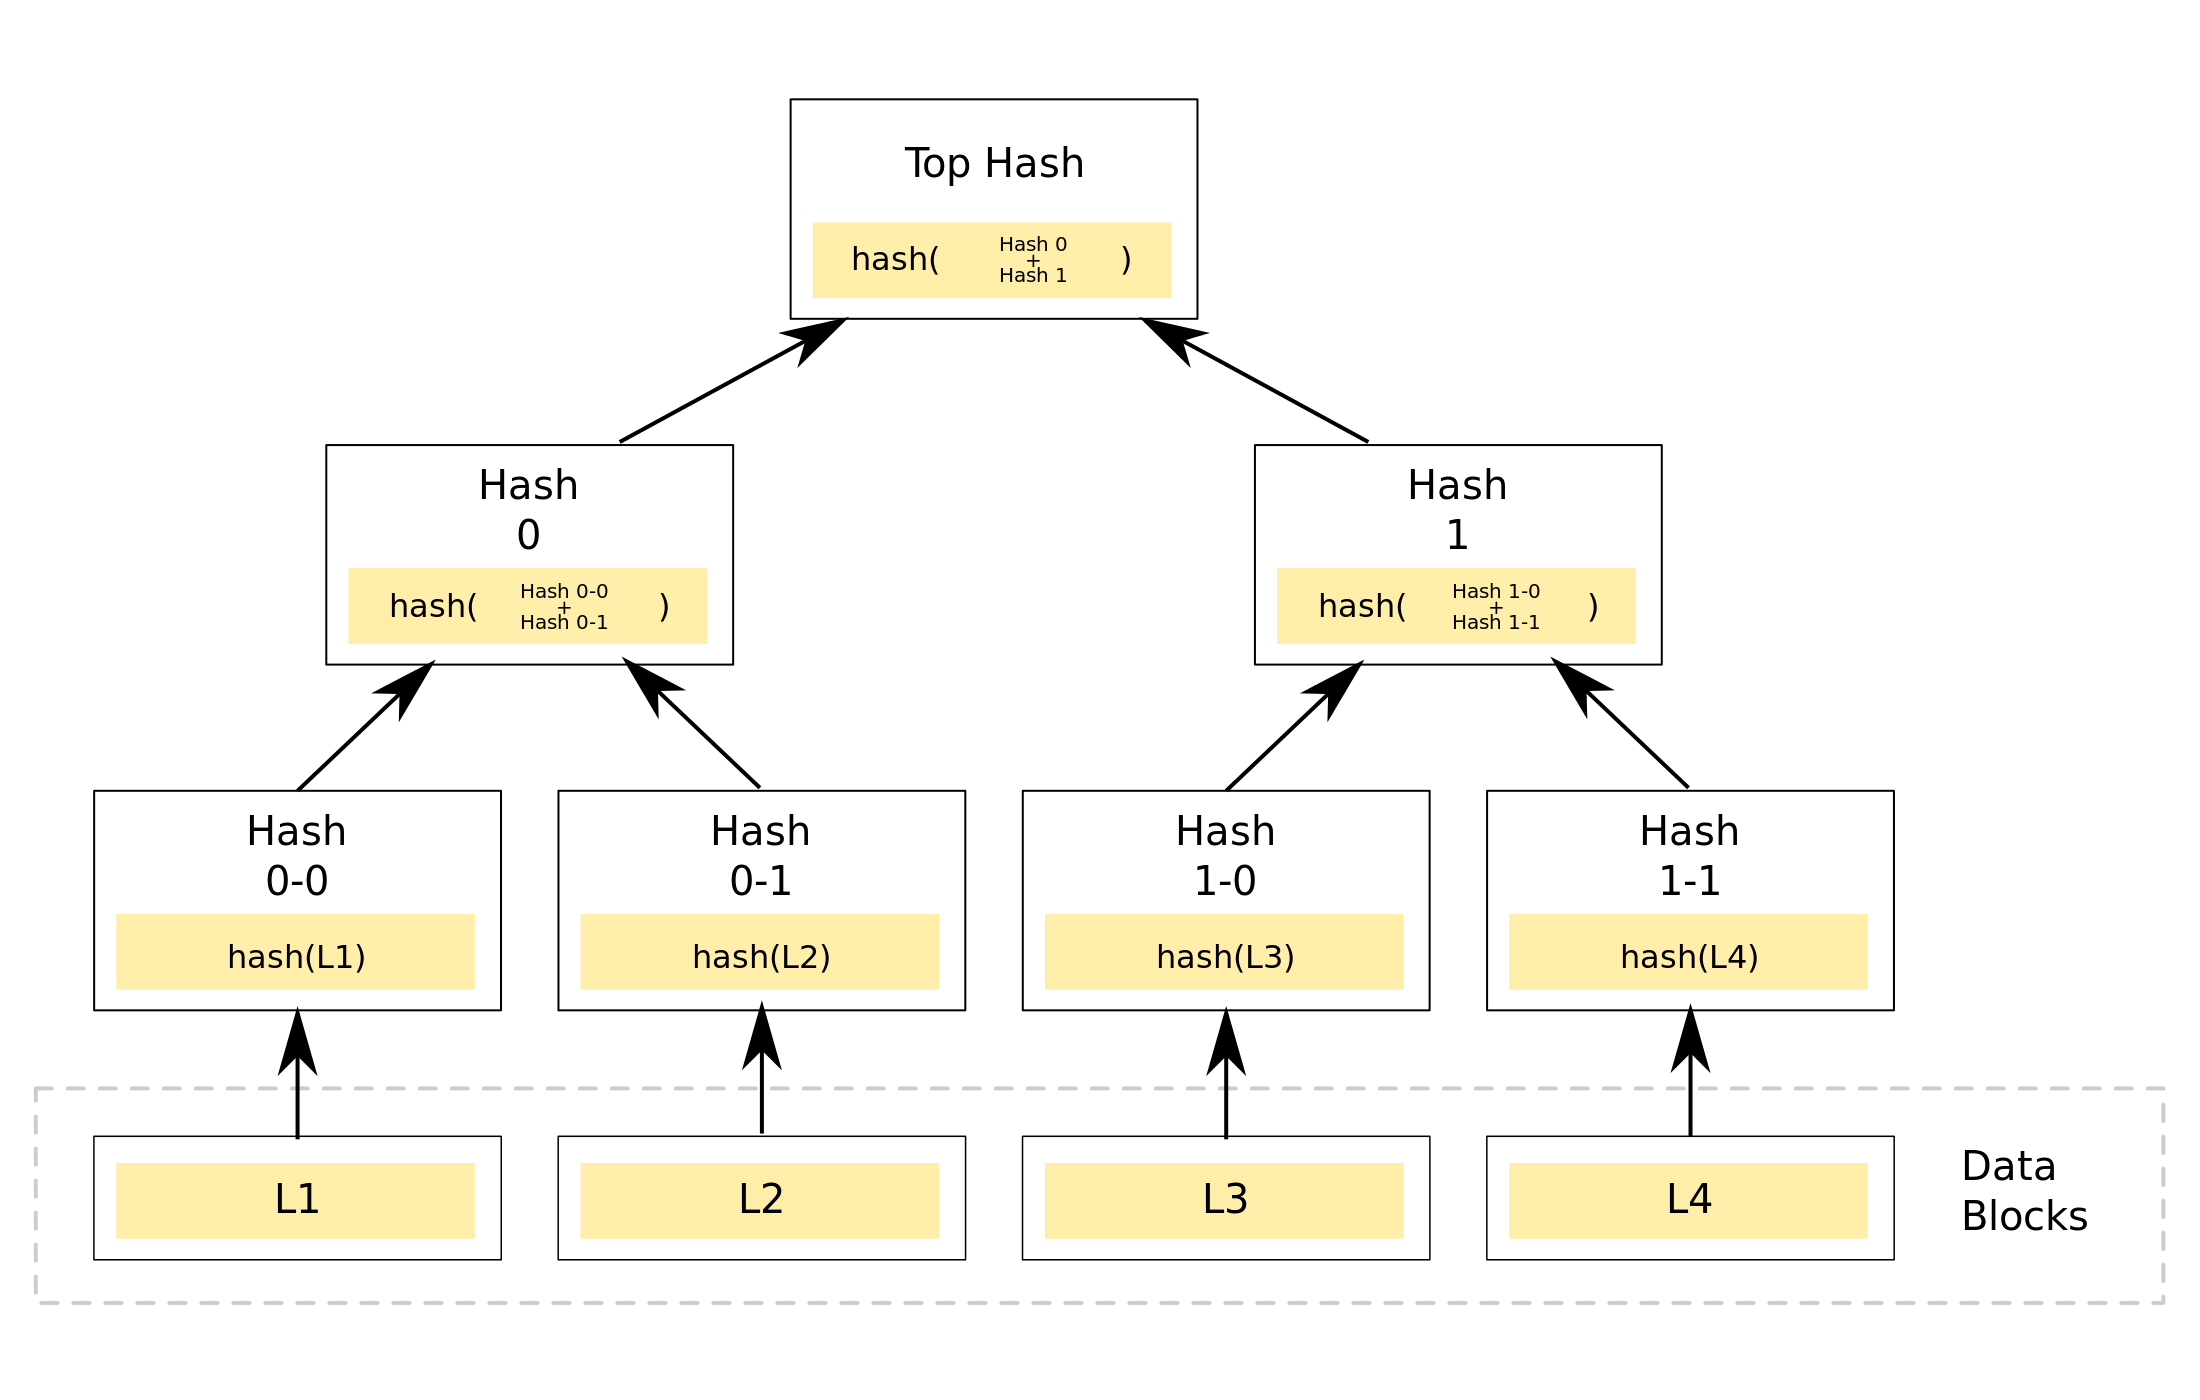
\includegraphics[width=.7\linewidth]{Hash_Tree.png}
 	\caption {یک درخت مرکل}
 	\label{fig:merkle}
 \end{figure}
 
 \subsection{انواع زنجیره‌ی قالبی}
 در این تحقیق زنجیره‌ی قالبی‌ها را از دو نظر دسته‌‌بندی می‌کنیم. زنجیره‌ی قالبی‌ها می‌توانند عمومی یا خصوصی باشند، در زنجیره‌ی قالبی‌های عمومی اضافه‌کردن بلوک به زنجیره‌ی قالبی دسترسی خاصی نمی‌خواهد و هر کسی می‌تواند در آن‌ها بنویسد ولی در زنجیره‌ی قالبی‌های خصوصی اضافه کردن بلوک صرفا توسط افراد خاص ممکن است. 
 \\
 روش دیگر تقسیم‌بندی ما باز یا بسته بودن زنجیره‌ی قالبی است که این دسته‌بندی در مورد دسترسی خواندن اطلاعات از زنجیره‌ی قالبی است. در زنجیره‌ی قالبی‌های بسته خواندن اطلاعات توسط عموم آزاد نیست و در زنجیره‌ی قالبی‌های خصوصی تمام اطلاعات زنجیره‌ی قالبی برای خواندن، در دسترس عموم است. 
\par
با توجه به کاربرد زنجیره‌ی قالبی مورد نظر هر زنجیره‌ی قالبی می‌تواند در هر کدام از این دسته‌بندی‌ها قرار بگیرد، جدول  \ref{tab:tch} یک کاربرد ممکن برای هر کدام از این دسته‌بندی‌ها را نشان می‌دهد.

\begin{table}[h]
	\begin{center}
		%		\def\arraystretch{2}
		\caption{انواع زنجیره‌ی قالبی}
		\begin{tabular}{|c|c|c|}
			\hline
			& باز & بسته \\
			\hline
			عمومی & ارز‌های دیجیتال & بعضی رای‌گیری‌ها \\
			\hline
			خصوصی & سامانه‌ی مدیریت اطلاعات مالیات & اطلاعات خصوصی یک شرکت \\
			\hline

		\end{tabular}
		\label{tab:tch}
	\end{center}
\end{table}


 
 
\section{اثبات‌های بی‌دانش}
اثبات‌ بی‌دانش 
\LTRfootnote{Zero knowledge proofs}
روشی است که یک «اثبات‌کننده» می‌تواند یه یک «بررسی‌کننده» نشان دهد که او یک راز - مثلا خروجی یک عملیات کامپیوتری - را می‌داند، بدون این که به بررسی‌کننده هیچ اطلاعات اضافه‌ای، مانند خروجی عملیات، بدهد. به عبارت دیگر اثبات‌های بی‌دانش، صرفا داشتن اطلاعات را اثبات می‌کنند و خود اطلاعات را محفوظ نگه‌ می‌دارند.
\\
یک اثبات بی‌دانش باید ۳ شرط زیر را داشته باشد:
\begin{itemize}
	\item
	کامل‌بودن: اگر گزاره‌ی مورد اثبات صحیح باشد، بررسی‌کننده‌ای که پروتکل را رعایت کند، باید از درستی گزاره مطمئن شود.
	\item 
	درستی: اگر گزاره مورد اثبات غلط باشد، هیچ اثبات‌کننده‌ای نتواند اثباتی ارائه کند که گزاره درست است. 
	\item 
	بی‌دانش: اگر اثبات درست باشد، بررسی کننده هیچ اطلاعاتی فراتر از این که گزاره درست است دریافت نکند.
\end{itemize}
اثبات‌های بی‌دانش، اثبات‌های احتمالاتی هستند و در واقع احتمال کمی وجود دارد که بتوان یک اثبات نادرست ارائه کرد. به بیان دیگر شرط درستی این است که احتمال تولید یک اثبات نادرست بسیار کم باشد. 
\subsection{مثال شهودی}
سناریویی را در نظر می‌گیریم که یک توپ سبز و یک توپ قرمز روی یک میز قرار دارد و آلیس می‌خواهد به باب که کوررنگ سبز و قرمز است ثابت کند که که این دو توپ با هم تفاوت دارند. برای اثبات آلیس چشمش را می‌بندد و باب یا دو توپ را جابجا می‌کند و یا جابجا نمی‌کند. در ادامه آلیس می‌گوید که آیا جای توپ‌ها با هم عوض شده‌اند یا نه. با یک پاسخ درست باب می‌فهمد که آلیس با احتمال ۵۰٪ درست می‌گوید. این فرایند را برای بار دوم نیز تکرار می‌کنند و در صورتی درستی جواب آلیس، باب می‌داند که با احتمال ۷۵٪ آلیس تفاوتی بین دو توپ می‌بیند. این فرایند آنقدر تکرار می‌کنند که باب با احتمال دلخواه خود از ادعای آلیس اطمینان پیدا کند.
\par
یک نکته‌ی مهم در مثال بالا این است که حتی اگر باب این فرایند را ضبط کرده باشد، نمی‌تواند به کس دیگری اثبات کند که آلیس تفاوت این دو توپ را می‌داند چون که راهی برای اثبات این که سوال و جواب از قبل هماهنگ نشده بوده است ندارد. 
\\
این یکی از نیازمندی‌های بی‌دانش بودن اثبات است. اگر در فرایند برای تصمیم‌گیری در تعویض توپ‌ها باب از شیر یا خط کردن یک سکه استفاده می‌کرد، دیگر این اثبات بی‌دانش نبود، چرا که باب می‌توانست با ضبط کردن این فرایند به یک شخص ثالث اثبات کند که آلیس تفاوت این دو توپ را می‌داند. 
\\
برای داشتن شرط بالا یک اثبات بی‌دانش همواره تعامل از سمت بررسی‌کننده نیاز دارد. اما با ریلکس کردن این شرط و استفاده از یک ورودی غیرقابل پیشبینی برای تولید سوال‌های یک اثبات بی‌دانش - مثلا هش ریشه‌ی یک درخت مرکل - می‌توان اثبات‌های بی‌دانش بدون نیاز به تعامل بررسی‌کننده ساخت. 


\subsection{اثبات‌های بی‌دانش بدون تعامل} 
منظور از اثبات بدون تعامل، اثباتی‌ است که در آن نیازی به فرستادن پیامی از سمت بررسی‌کننده به اثبات‌کننده نباشد. با این روش‌ها اثبات‌کننده می‌تواند اثبات را مستقل از بررسی‌کننده بسازد و ارسال کند، در ادامه‌ی این تحقیق اثبات‌های بی‌دانش و بی‌تعامل را 
\textbf{شاهد}
می‌نامیم. در ادامه دو روش تولید یک شاهد بی‌دانش را بررسی می‌کنیم. این روش‌ها می‌توانند برای خروجی هر محاسبات کامپیوتری شاهد ایجاد کنند. 

\subsubsection{اثبات بی‌دانش \lr{ZK-SNARK}}
یکی از پرکاربردترین روش‌های ایجاد شاهد 
\lr{ZK-SٔNARK}
\LTRfootnote{Zero-Knowledge Succint Non-Interactive Argument of Knowlege}
\cite{zksnark}
است. شاهد‌های این روش علاوه بر بی‌دانش بودن ویژگی‌های زیر را دارند:
\begin{itemize}
	\item 
	مختصر
	\LTRfootnote{Succinct}
	: تولید و بررسی شاهد از انجام خود محاسباتی که اثبات می‌شود کوتاه‌تر (معمولا از مرتبه‌ی زمانی $ (\log N) ^ 2$) است. 
	\item
	بی‌تعامل
	\LTRfootnote{Non-Interactive}
	: نیازی به پیامی از بررسی‌کننده برای ایجاد شاهد نیست. 
	\item
	ادعای دانش
	\LTRfootnote{Argument of Knowledge}
	: اثبات ارائه شده در این روش درست 
	\LTRfootnote{Sound}
	است و نمی‌شود بدون داشتن اطلاعات آن را در زمان محدود ساخت.
	
\end{itemize}
 
\begin{figure}[bh]
	\centering
	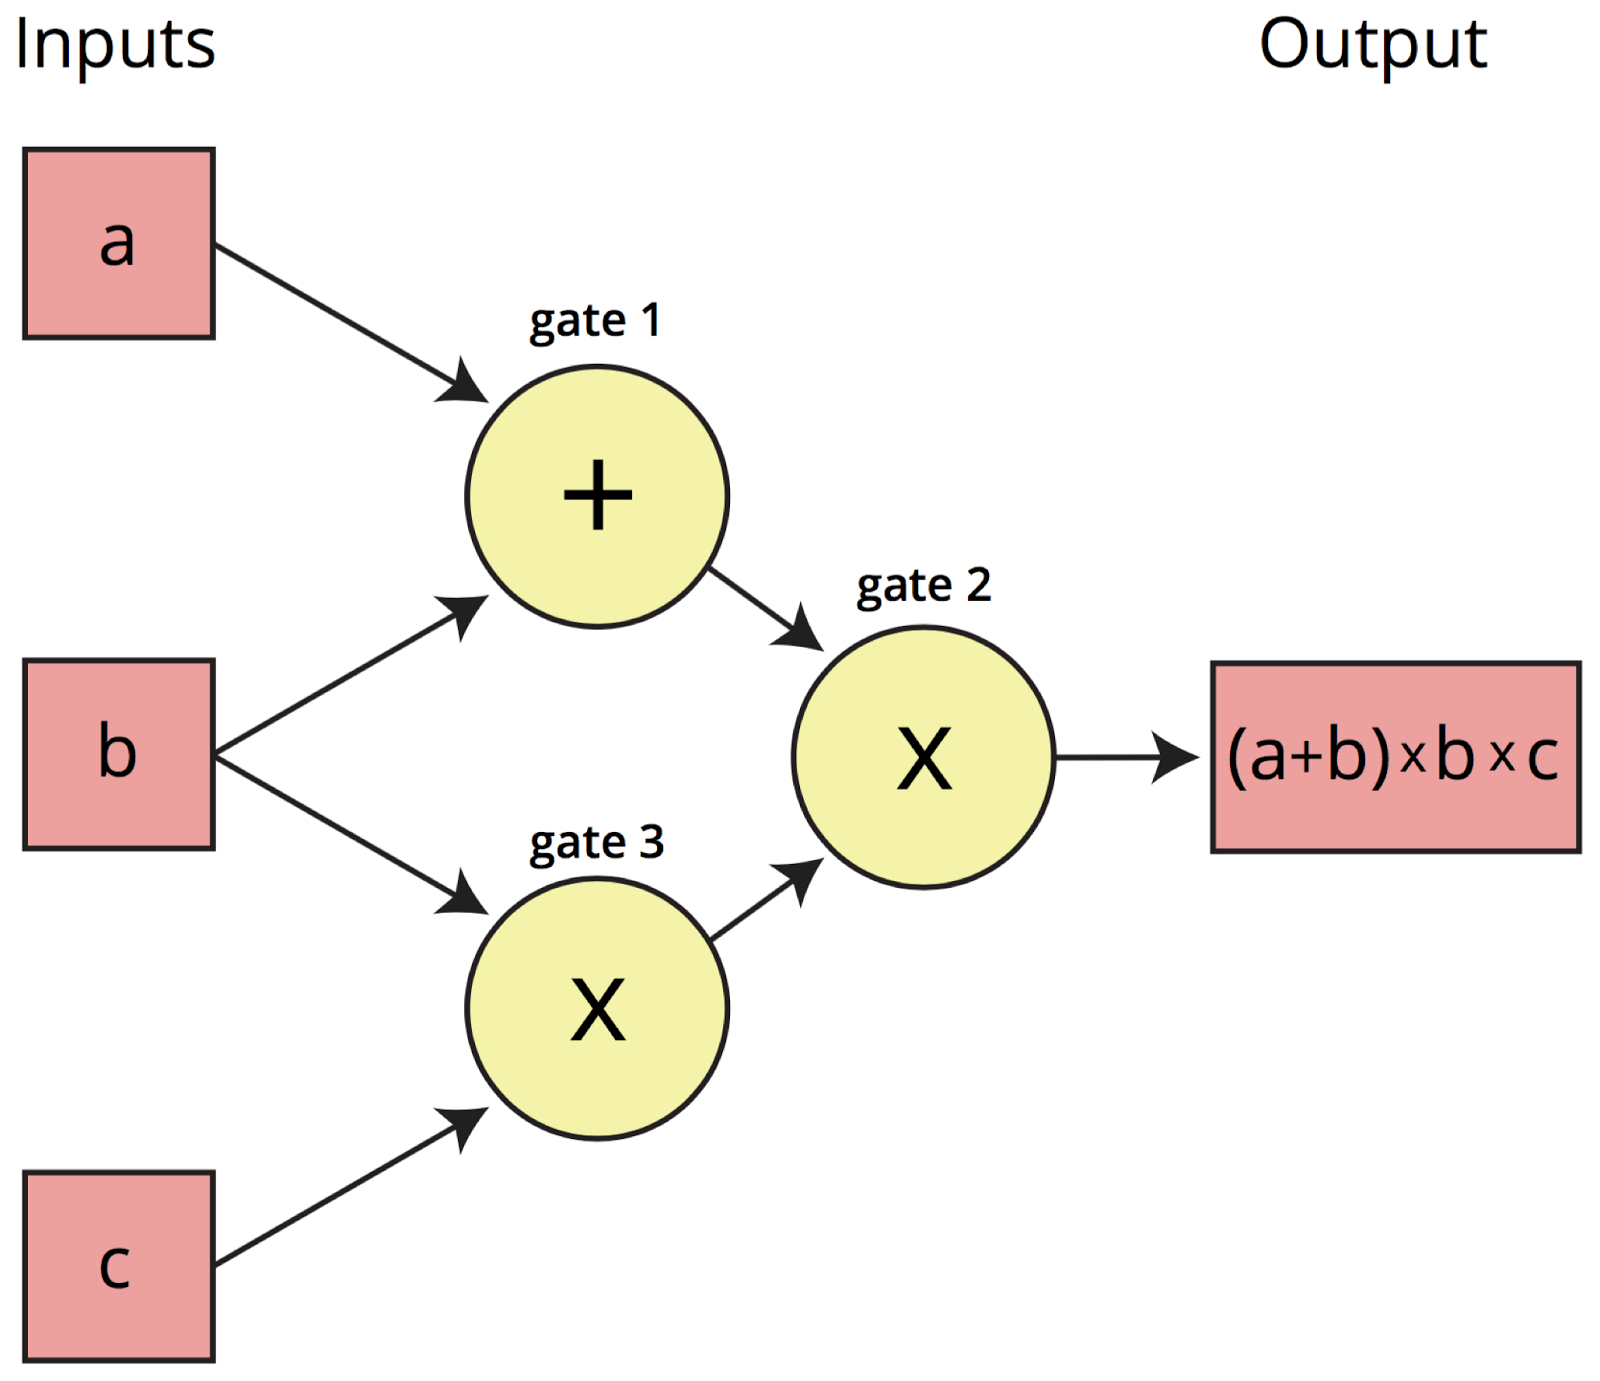
\includegraphics[width=.5\linewidth]{arithmetic-circuit.png}
	\caption {یک نمونه مدار محاسباتی}
	\label{fig:arithmetic}
\end{figure}

برای ساختن یک شاهد به این روش ابتدا محاسبات لازم را به یک مدار محاسباتی ریاضی تبدیل می‌کنیم به طوری که اثبات را به عنوان تعدادی شرط روی این مدار نشان دهیم، سپس به کمک یک
\lr{elliptic curve}
مقدار مدار را در چند نقطه‌ی تصادفی به عنوان اثبات ارائه می‌کنیم، با صادق بودن شرط‌ها در این نقاط شاهد را بررسی می‌کنیم. 
\\
برای انتخاب یکسان این نقاط تصادفی بین اثبات‌کننده و بررسی‌کننده نیاز به تعدادی نقطه‌ی توافق شده روی \lr{elliptic curve} داریم که باید در قبل از تولید اثبات انتخاب شده باشند. در این فاز آماده‌سازی تعدادی عدد تصادفی برای انتخاب این نقاط تولید می‌شوند که بعد از تولید نقاط باید بلافاصله پاک شوند. کسی که این اعداد (در واقع نقطه‌ی شروع روی منحنی) را داشته باشد می‌تواند شاهد‌های تقلبی ایجاد کند. برای تولید شاهد واقعی نیازی به دانستن این نقاط نیست و بنابراین بعد از فاز آماده‌سازی این اعداد باید پاک شوند. 
\subsubsection{اثبات بی‌دانش \lr{ZK-STARK}}
از روش‌های دیگر ایجاد شاهد بی‌دانش روش \lr{ZK-STARK}
\LTRfootnote{Zero-Knowledge Scalable Transparent ARguments of Knowledge}
\cite{zkstark}
است. مهم‌ترین وجه تمایز این روش در مقایسه با
\lr{ZK-SNARK}
 «شفافیت»
 \LTRfootnote{Transparency}
است، به این معنی که نیازی به فاز آماده‌سازی ندارد. عدم نیاز به آماده‌سازی و نداشتن زباله‌ی سمی (اطلاعاتی که باید پاک شوند تا امنیت سیستم تامین شود) این روش را برای کاربرد‌های حساس مناسب‌تر می‌کند اما در ازای این امنیت، حجم شاهد‌ها از چند صد بایت به چند صد هزار بایت تغییر می‌کند.
\par
ار مزیت‌های دیگر این روش استفاده نکردن از 
\lr{Elliptic curve}ها
است. نیاز‌های کم این روش باعث می‌شود که حتی با کامپیوتر‌های کوانتمی
\LTRfootnote{Quantum computers}
 راهی برای شکستن این اثبات‌ها وجود نداشته باشد.
\\
برای ساختن یک شاهد با این روش، برنامه‌ی مورد نظر را تبدیل یه یک چندچمله‌ای درجه بالا می‌کنند، سپس از مقدایر این چندجمله‌ای یک درخت مرکل ساخته می‌شود که مقدایر مختلف خروچی را نشان می‌دهد. سپس بررسی‌کننده چند شاخه از این درخت را به طور تصادفی انتخاب و بررسی می‌کند. برای غیرتعاملی کردن این اثبات می‌توان از هش ریشه‌ی درخت مرکل به عنوان ورودی یه تابع شبه‌تصادفی
\LTRfootnote{Pseudo random}
استفاده می‌شود که مشخص می‌کند خروجی کدام شاخه‌ها باید در شاهد بیاید. 





\cchapter{کارهای پیشین}

از آن‌جایی که مهمترین خصوصیت‌های یک سیستم رای‌گیری مناسب امنیت شمارش آرا و حفظ حریم خصوصی رای‌دهنده است، این دو موضوع پایه‌های طراحی سیستم ما خواهند بود. سیستم‌های رای‌گیری الکترونیک قبل از تکنولوژی زنجیره‌ی قالبی از روش‌های متعددی برای تحقق این هدف استفاده می‌کردند اما تقریبا در تمامی این روش‌ها نیاز به اعتماد به مجری انتخابات وجود دارد. 
\par
طراحی زنجیره‌های قالبی همراه به کمک روش‌های توافق خلاقانه باعث ایجاد ارز‌های دیجیتال بدون نیاز به یک شخص (بانک) مورد اعتماد شد. در ادامه این ساختارداده‌ی اکیدا افزایشی برای حذف نیاز به اعتماد در کاربدهای دیگر نیز استفاده شده است. زنجیره‌ی قالبی در این تحقیق نیز به عنوانی ابزاری که با ایجاد شفافیت نیاز به اعتماد را کاهش می‌دهند استفاده می‌شود.
\par 
شفافیت در انتخابات خود باعث ایجاد مشکلاتی برای امنیت رای‌دهندگان می‌شود. عدم حفظ حریم خصوصی رای‌دهنده در یک انتخابات می‌تواند باعث شود رای‌دهنده نتواند به کاندیدای دلخواهش رای دهد یا تحت فشار مجبور به رای‌دادن شود. برای رفع این مسئله از روش‌هایی مانند اثبات‌های بی‌دانش استفاده می‌شود. اثبات‌های بی‌دانش این امکان را ما می‌دهند تا بتونیم حتی با حفظ حریم خصوصی کاربر، درستی شمارش انتخابات را اثبات کنیم.


\section{رای‌گیری الکترونیک}
رای‌گیری الکترونیک را به طور کلی می‌توانیم به دو دسته‌ی رای‌گیری تماما الکترونیک و رای‌گیری به کمک ابزار‌های الکترونیکی تقسیم کرد. روش‌های دسته‌ی دوم مبتنی بر رای‌گیری سنتی هستند و از ابزاری‌های الکترونیکی صرفا برای کاهش هزینه و افزایش دسترسی پذیری استفاده می‌کنند. از این روش‌ها می‌توان به ابزارهای شمارش رای خودکار و یا دستگاه‌های ثبت رای‌الکترونیکی که خروجی آن‌ها یک برگه‌ی رای‌ کاغذی
\LTRfootnote{Direct-recording electronic voting systems (DRE)}
است اشاره کرد. در این تحقیق این ابزارها را بررسی نمی‌کنیم و منظور از رای‌گیری الکترونیک، دسته‌ی اول یا رای‌گیری تماما الکترونیک است.
\par
سیستم‌های رای‌گیری الکترونیک را می‌توان به دو دسته‌ی کلی توزیع‌شده و متمرکز تقسیم کرد. سیستم‌های متمرکز نیازمند یک ارتباط امن از رای‌دهنده تا سرویس مرکزی هستند. همچنین نیازمند اعتماد کامل به همان یک سرویس برای درستی انتخابات است. در سیستم‌های توزیع‌شده تلاش می‌کنند تا این دو مسئله را کمرنگ‌تر کنند.

\subsection{رای‌گیری الکترونیک متمرکز}
در این سیستم‌ها یک سامانه‌ی مرکزی وجود دارد که تمامی آرا در آن زخیره می‌شند. در این سیستم‌ها حوزه‌های رای‌گیری می‌توانند وجود داشته باشند اما حوزه‌ها صرفا وظیفه‌ی احراز هویت و ارائه‌ی درگاه امن برای ثبت رای در سامانه‌ی مرکزی را دارند. حریم خصوصی کاربران در این سیستم‌ها مبتی بر استفاده از کانال‌های ارتباطی ناشناس 
\LTRfootnote{Anonymous communication channel}
بین حوزه‌های رای‌گیری و سامانه‌ی مرکزی است.
\par
اولین تحقیق در رابطه با استفاده‌ از کانال‌های ارتباطی ناشناس برای رای‌گیری در سال ۱۹۸۵ توسط 
\lr{Chaum}
\cite{Chaum}
بود، که در آن برای ساخت‌ کانال‌های ارتباطی ناشناس از امضای کورکورانه 
\LTRfootnote{Blind signature}
\cite{blindsig}
برای ایجاد یک ارز دیجیتل استفاده می‌شد. در امضای کورکورانه، برای حفظ حریم خصوصی تاییدکننده‌ی اطلاعات، رمزشده‌ی اطلاعات را امضا می‌کند، به این صورت از اطلاعات پیام باخبر نمی‌شود. اولین تلاش برای ایجاد یک پروتکل رای‌گیری الکترونیک با امضای کورکورانه در سال ۱۹۹۲ 
\cite{foo92}
بود و در ادامه در سال ۱۹۹۷
\cite{improveblind}
نسخه‌ی کامل‌تری از آن ارائه شد. این روش‌ها مبتنی بر وجود یک شمارنده و یک حوزه هستند، حوزه احراز هویت را انجام می‌دهد و برگه‌ رای‌های ناشناس صادر می‌کند و سپس از طریق یک کانال ارتباطی ناشناس رای‌دهنده رای را به شمارنده می‌دهد. از مشکلات این روش می‌توان به نیاز به اعتماد به حوزه اشاره کرد. حوزه می‌تواند که با ارائه رای‌های اشتباه بدون توانایی پیگیری، رای‌گیری را خراب کند، برای حل این مشکل تحقیقاتی
\cite{multiteller}
در راستای استفاده از چند حوزه انجام شده است. مشکل بزرگ دیگر این روش‌ها
\cite{anonchan}
سختی ناشناس نگه‌داشتن کانال‌های ارتباطی ناشناس است.

\subsection{رای‌گیری الکترونیک توزیع‌شده}
رای‌گیری الکترونیک توزیع‌شده را به سه دسته‌ی رای‌گیری‌های بدون زنجیره‌ی قالبی، با زنجیره‌ی قالبی عمومی و با زنجیره‌ی قالبی خصوصی تقسیم می‌کنیم. با توجه به این که در رای‌گیری احرازهویت یک مسئله‌ی مهم است همه‌ي این سیستم‌ها از زنجیره‌ی قالبی‌های بسته استفاده می‌کنند.
\subsubsection{رای‌گیری بدون زنجیره‌ی قالبی} 
بعضی سیستم‌های طراحی شده برای رای‌گیری الکترونیک
\cite{secret1}
\cite{secret2}
\cite{secret3}
از روش‌های تقسیم راز
\LTRfootnote{Secret sharing}
استفاده می‌کنند. در این روش‌ها فرایند ثبت رای باید به تایید تعدادی از حوزه‌ها برسد که باعث کاهش نیاز به اعتماد می‌شود. در این روش‌ها می‌توان اثبات کرد که برای ردیابی یک رمز حداقل $k$ حوزه باید تبانی کنند. مشکل بزرگ این روش‌ها عدم وجود یک الگوریتم مقیاس‌پذیر برای تقسیم راز است.
\par
روش دیگری که برای رای‌گیری توزیع‌شده استفاده شده است، استفاده از بردار‌ بررسی
\LTRfootnote{Check vector}
\cite{checkvector}
است. در این روش‌ها بررسی درستی رای‌ها کاملا توزیع‌شده‌ است، اما نیاز به ارتباط دو به دوی تمامی رای‌دهنده‌ها دارد که در یک انتخابات واقعی شدنی نیست. ترکیبی از این روش و تقسیم راز باعث ایجاد پروتکل‌هایی
\cite{MPO1} \cite{evotinwocrypto}
شد که با سطح‌بندی حوزه‌ها و تقسیم رای‌ها و مخلوط کردن آن‌ها از حریم خصوصی حمایت می‌کنند، اما این روش‌ها به حوزه‌ها و رای‌دهندگان توانایی بررسی درستی برگه رای‌ها را نمی‌دهد و امکان ایجاد رای‌های اشتباه و جلوگیری از رای‌دادن یک فرد خاص را ایجاد می‌کنند. 


\subsubsection{رای‌گیری با زنجیره‌ی قالبی عمومی}
با فراگیر شدن تکنولوژی زنجیره‌ی قالبی
\cite{rosgood}
، محصولاتی در زمینه‌ی رای‌گیری الکترونیک به کمک این تکنولوژی ساخته شدند. تعدادی از این سیستم‌های رای‌گیری در قالب قرارداد‌های هوشمند
\LTRfootnote{Smart contract}
\cite{SmartContract}
ساخته‌ شده‌اند که از آن‌ها می‌توان به وتریم 
\LTRfootnote{Votereum}
\cite{votereum}
و یا سامانه‌ی ارائه شده توسط
\lr{E.Yavuz}
\cite{yavuz}
در بستر اتریوم
\LTRfootnote{Ethereum}
\cite{Ethereum}
- که یک ارز دیجیتال و یک بستر قرارداد هوشمند است - 
اشاره کرد. مزیت این نوع رای‌گیری‌ها هزینه‌ی اولیه کم برای استفاده از آن‌هاست، اما همچنین خطر اشتباه برنامه‌نویسی
\cite{surveyAtt}
\cite{gyges} \cite{smart}
در این سبک کارها بسیار بالاست. همچنین هزینه اجرای قراردادهای هوشمند به تعداد بالا برای یک رای‌گیری هزینه‌ی بالایی خواهد داشت که در طول زمان باعث افزایش هزینه‌های رای‌گیری خواهد شد. مسئله‌ی دیگر در بستر اتریوم هم وابستگی سیستم رای‌گیری، به پهنای باند نود‌های اتریوم و میزان بار روی شبکه‌ی آن است. این موضوع می‌تواند باعث کند شدن یا حتی در مواردی حذف شدن تعدادی از آرا شود.

\subsubsection{ٰرای‌گیری با زنجیره‌ی قالبی خصوصی}
از سیستم‌های رای‌گیری با زنجیره‌ی قالبی خصوصی می‌توان به 
\lr{VoteBook}
\cite{votebook}
توسط شرکت 
\lr{Kaspersky}
که یک شرکت پیشرو در زمینه‌ی امنیت است اشاره کرد. فلسفه‌ی ساخت این سیستم به صورتی است که تلاش می‌کند برای کاربرانی که از سیستم‌هایی رای‌گیری فعلی استفاده می‌کنند کمترین تغییر در رفتار نیاز باشد. 
\\
از مثال‌های دیگر سیستم‌های رای‌گیری مبتنی بر زنجیره‌ی قالبی می‌توان به استارت‌آپ 
\lr{Follow My Vote}
اشاره کرد. نحوه‌ی کار این سیستم با  
\lr{VoteBook}
تفاوت اساسی دارد و برای رای‌دادن احتیاج است که نرم‌‌افزاری به روی کامپیتور و یا تلفن‌همراه کاربران نصب شود. این روش طراحی سیستم،‌ خطرات امنیتی در قالب بدافزار ایجاد می‌کند. همچنین با نبود یک حوزه‌ی رای‌گیری امن راهی برای تامین امنیت رای‌دهندگان و اطمینان حاصل کردن از این که کسی مجبور به رای‌ دادن نشده، نیست.
\\
یکی از موفق‌ترین سیستم‌های رای‌گیری مبتنی بر زنجیره‌ی قالبی موجود در حال حاضر 
\lr{VoteWatcher}
ساخته شده توسط یک شاخه از شرکت 
\lr{blockchain Technologies Corporation}
است که یک شرکت بزرگ برای ارائه‌ی سرویس‌های مبتنی بر زنجیره‌ی قالبی است. طبق وب‌سایت این محصول تاکنون بیش از صدهزار رای در بیشتر از ۲۰ رای‌گیری مختلف توسط این سیستم‌ شمارش شده‌است. 
\\
مدل اسفاده‌ی 
\lr{VoteWatcher}
به سیستم‌ 
\lr{VoteBook}
بسیار شبیه است و تفاوت رفتاری زیادی با مدل‌های رای‌گیری الکترونیکی فعلی برای کاربران ندارد. در این محصول طبق نیاز رای‌گیری می‌توان از یک زنجیره‌ی قالبی عمومی یا خصوصی استفاده کرد.
\\
از موارد دیگر می‌توان به پیاده‌سازی‌های به کمک قرارداد‌های هوشمند ولی با استفاده از زنجیره‌ی قالبی خصوصی 
\cite{privblock}
که توانایی ردگیری بالاتری از پیاده‌سازی‌های دیگر ارائه می‌کنند، اشاره کرد اما به دلیل کندی نسبی، نیاز به تقسیم رای‌گیری به چند رای‌گیری کوچک‌تر دارند.


\section{اعتماد}
همانطور که اشاره کردیم برای ایجاد یک رای‌گیری خوب تا جای ممکن باید نیاز به وجود شخص معتمد را حذف یا حداقل کم‌رنگ کنیم. ساده‌ترین راه‌حل برای حذف نیاز به اعتماد ایجاد شفافیت و عمومی ساختن تمامی اطلاعات است؛ در صورتی که همه بتوانند تمامی اطلاعات را بررسی کنند و از درستی آن‌ها اطمینان حاصل کنند، دیگر نیازی به اعتماد کردن به شخص دیگر ندارند. 
\par 
با استفاده از زنجیره‌ی قالبی می‌‌توانیم برای بررسی درستی اطلاعات همواره با بررسی بلوک آخر از درستی کل زنجیره اطمینان حاصل کنیم اما با توجه این که چندین نفر می‌توانند به آن بلوک اضافه کنند ممکن است سناریویی پیش بیاید که در آن دو یا چند نسخه‌ی درست از زنجیره‌ی قالبی وجود داشته باشد. برای حل این مسئله باید پروتکلی داشته باشیم که یا اجازه‌ی پیش آمدن این شرایط را ندهد و یا روشی برای حذف تعدادی از آن‌ها ارائه کند و کاری کند که در طول زمان پس از مدتی فقط یک نسخه‌ی درست از زنجیره‌ی قالبی باقی بماند. این پروتکل را روش توافق می‌نامیم.
\subsection{روش توافق}
توصیف رسمی این مسئله، مسئله‌ی ژنرال‌های بیزنتین 
\LTRfootnote{The Byzantine genarals problem}
\cite{byzantine}
است. در این مسئله چند ژنرال که می‌توانند یک به یک با هم صحبت کنند، در تلاشند تا به توافق برسند که آیا باید حمله کنند یا نکنند، تعدادی از ژنرال‌ها خائن هستند و در تلاشند که نتیجه‌ی توافق ژنرال‌ها را تغییر دهند. ژنرال‌های خائن می‌توانند با جواب ندادن یا جواب غلط دادن تلاش کنند که نتیجه‌ی توافق را تغییر دهند. در ساده‌ترین حالت و بدون استفاده از امضا‌های دیجیتال ثابت می‌شود که برای $ 3k + 1 $ ژنرال، با رای‌گیری می‌توان تا $ k $ خائن را تحمل کرد. 
\par
راه‌حل‌های متعددی برای توافق 
\LTRfootnote{اثبات‌ کار}
در بستر زنجیره‌ی قالبی داده شده که در ادامه به تعدادی از آن‌های می‌پردازیم.
\subsubsection{توافق در ارزهای دیجیتال}
روشی که 
\lr{S.Nakomoto}
\cite{bitcoin}
برای رفع این مسئله در بیت‌کوین استفاده کرده است، اثبات کار 
\LTRfootnote{Proof of work}
نام دارد. این روش که بر پایه‌ی روش استفاده شده در 
\lr{hashcash}
\cite{hashcash}
است. در این روش برای اضافه شدن هر بلوک به زنجیره‌ی قالبی باید یک مسئله‌ی سخت (که نیاز به توان پردازشی بالا دارد) حل شود ولی بررسی درستی جواب ساده است. این روش روش بسیار فراگیری در ارز‌های دیجیتال است. از مشکلات این روش می‌توان به توان مصرفی بالا و کندی نسبی آن اشاره کرد. برای مثال حداکثر توان تئوری بیت‌کوین، ۷ تراکنش بر ثانیه است. 
\subsubsection{اثبات سهم}
در روش اثبات سهم
\LTRfootnote{proof of stake}
\cite{PoS}
برای ساخت بلوک‌های جدید باید یک فاکتور مقدار سکه‌های در اختیار ماینتر و سن آن‌هاست. به این صورت که می‌تواند در ازای سن‌ سکه‌های در اختیارش (با زدن یه تراکنش به خود) هش ساده‌تری برای بلوک بعدی اعمال کند. مزیت اصلی این روش توان مصرفی پایین‌تر آن به نسبت اثبات کار است. 
\\
معمولا در زنجیره‌ی قالبی‌ها در بلوک‌های ابتدایی ار روش اثبات کار استفاده می‌شود و بعد از مدتی برای کاهش هزینه‌های اضافه کردن بلوک چدید و مقیاس‌پذیری می‌توان از این روش یا ترکیب این روش‌ها استفاده کرد.

\subsubsection{\lr{Ripple Consensus Protocol}}
در این روش
\cite{ripple} \cite{ripple2}
 تعدادی شخص مورد اعتماد وجود دارند که برای اضافه‌شدن بلوک به زنجیره‌ی قالبی باید درصدی از آن‌ها درستی تراکنش را تایید کنند. این اشخاص در دسته‌های مختلف قرار می‌گیرند و برای تایید باید یک زیردسته‌ی کامل تراکنش‌ها را تایید کنند.
 \\
 با وجود سرعت نسبتا بالای این روش - تا ۱۰۰۰ تراکنش در ثانیه - منتقدین آن از نیاز به اشخاص مورد اعتماد می‌گویند. این روش تا $ n /5 $ خطا در نود‌های مورد اعتماد را می‌تواند تحمل کند.


\subsubsection{\lr{Stellar Consensus Protocol}}
 روش 
\lr{SCP}
\cite{scp}
 مبتنی بر ایجاد افراد مورد اعتماد، به صورت طبیعی و خودجوش، در شبکه است. در این روش با افزایش تراکنش‌های درست توسط هر شخصی، آن شخص به عنوان فرد مورد اعتماد شناخته می‌شود و هر تراکنش را باید تعداد افراد مورد اعتماد تایید کنند. این افراد توسط پرداخت‌کننده‌ی تراکنش انتخاب می‌شوند اما دسته‌بندی آن‌ها در شبکه‌ به گونه‌ای است که خطا در تایید تراکنش باعث حذف شدن فرد از لیست افراد مورد اعتماد شود. تفاوت اصلی این روش با 
 \lr{Ripple}
 در توانایی انتخاب تاییدکنندگان تراکنش است و فرض‌های اعتماد کمتر این روش باعث می‌شود که تا $ n /3 $ خطا در نود‌های مورد اطمینان را بتواند تحمل کند.
\section{اثبات‌های بی‌دانش}
اثبات‌های بی‌دانش اولین بار در سال ۱۹۸۵ 
\cite{GHY}
به عنوان روشی ساخت یک روش رمزنگاری متقارن با کلید عمومی استفاده شد. با پیشرفت تکنولوژی اثبات‌های بی‌دانش،‌ روش‌های جامع اثبات بی‌دانش مانند
\lr{ZK-SNARK} 
\cite{zksnark}
و \lr{ZK-STARK} 
\cite{zkstark}
بوجود آمدند. این روش‌ها توانایی اثبات هر محاسباتی را به صورت بی‌دانش دارند و این موضوع باعث استفاده‌ی آن‌ها در کاربردهای بیشتری شد.
\par
با توجه به این که 
\lr{ZK-SNARK}
، به طور خاص خاص پروتکل پینوکیو
\LTRfootnote{Pinocchio}،
فراگیرترین روش برای ایجاد اثبات‌های بی‌دانش است. تحقیقات زیادی در مورد فاز آماده‌سازی و ایجاد پارامترهای عمومی این مدل انجام شده است. همانطور که قبلا اشاره کردیم ورودی‌های این فاز اگر پس از استفاده‌ی اولیه پاک نشوند می‌توانند برای ایجاد اثبات‌های تقلبی استفاده شوند.
\par
از این تحقیق‌ها می‌توان به روش‌هایی
\cite{znsetup} \cite{multipartyparams}
که تلاش در کاهش نیاز به اعتماد در این فاز می‌کنند اشاره کرد. این روش‌ها باعث می‌شوند که برای لو رفت اطلاعات خطرناک احتیاج به تبانی تمامی اعضای موجود در فاز آماده‌سازی باشد.
\par
از دیگر کارهای در این زمینه می‌توان به تلاش‌هایی برای حذف فاز آماده‌سازی به طور کلی اشاره کرد. این روش‌ با تغییر اساسی در پروتکل و استفاده از چندجمله‌ای‌ها 
\cite{nosetup}
مرحله‌ي آماده‌سازی را حذف می‌کند
\subsection{کاربرد‌ها}
با فراگیری ارز‌های دیجیتال، مسئله‌ی حریم خصوصی در آن‌ها پررنگ‌تر شد. در ابتدا یکی از بزرگ‌ترین کاربردهای بیت‌کوین پرداخت‌های مجرمانه بود که ناشناسی نسبی در این بستر باعث می‌شد برای این سبک‌ پرداخت‌ها ایده‌آل باشند. اما به دلیل عمومی بودن زنجیره‌ی قالبی و تمامی تراکنش‌ها در آن دنبال کردن رد پرداخت بسیار ساده است.
\par
 برای جلوگیری از این ردگیری در کاربردهای مجرمانه از یک شخص مورد اعتماد برای «مخلوط کردن» سکه‌های افراد استفاده می‌شود. در این روش چندین نفر به یک نفر پرداخت می‌کنند و آن فرد به کلید‌های عمومی که از قبل تعیین شده با سکه‌های جدید پرداخت می‌کند اما در این روش همگی به شخص مخلوط کننده اعتماد می‌کنند که به اندازه پرداخت کند و رد واقعی سکه‌ها را جایی ثبت نکند. این روش برای کاربردهای مجرمانه تا حد بسیار خوبی پاسخگو است اما برای افراد عادی که صرفا دغدغه‌ی حریم خصوصی خود را دارند خطرها و هزینه‌ي این روش معقول نیست، به همین دلیل کارهای مختلفی در زمینه‌ی پرداخت ناشناس انجام شده است. 
 
\subsubsection{پرداخت ناشناس}
از این تحقیقات می‌توان به بستر 
\lr{HAWK}
\cite{hawk}
اشاره کرد. در این تحقیق به کمک یک تعریف کلی از زنجیره‌ی قالبی به عنوان سیستمی که همواره در دسترس است و هیچ اطلاعات اشتباه نمی‌پذیرد اما حریم خصوصی را حفظ نمی‌کند یک بستر قرارداد هوشمند ساخته شده است که در آن به ازای کد قرارداد هوشمند، یک کد برای حفظ حریم خصوصی به کمک اثبات‌های بی‌دانش ساخته می‌شود. روش کار این سیستم مبتنی بر ایجاد آدرس‌های مقصد یکتا به ازای هر تراکنش است. 
\\
مونرو 
\LTRfootnote{Monero}
که یک ارز دیجیتال است که بر اساس الگوریتم 
\lr{Cryptonote}
\cite{monero}
کار می‌کند، به مانند 
\lr{HAWK}
با یکتا سازی آدرس‌های مقصد و امضای حلقه‌ای 
\LTRfootnote{ًRing Signature}
کار می‌کند. در ادامه این ارز دیجیتال با همین روش مدلی 
\cite{monero2}
برای مخفی کردن پرداخت‌کننده‌ی سکه نیز ارائه کرد.
\par
از کارهای دیگر در این زمینه‌ می‌توان به 
\lr{zerocoin}
\cite{zerocoin}
که روش پرداخت ناشناس بر بستر بیت‌کوین به کمک 
\lr{ZK-SNARK}
ارائه کرد اشاره کرد. روش استفاده شده در آن با بهبود در ارز دیجیتال 
\lr{z-cash}
\cite{zerocash}
استفاده شد. این ارز دیجیتال دو مدل سکه‌ی قابل ردگیری و غیرقابل ردگیری دارد و هر کسی می‌توان طی یک تراکنش سکه‌های خود را به سکه‌های ناشناس تبدیل کند.



\cchapter{روش پیشنهادی}
روش پیشنهادی ما سه هدف کلی دارد: ۱- هر رای‌دهنده از شمارش درست رای خود اطمینان حاصل کند ۲- حریم خصوصی حفظ شود ۳- هر خطا در فرایند رای‌گیری قابل تشخیص باشد. برای رسیدن به این اهداف نیاز است باید فرایند به گونه‌ای طراحی شود که هیچ فردی معتمد فرض نشود. برای این کار ابتدا شرایط و فرضیات مسئله را به طور دقیق‌تر بررسی می‌کنیم، در ادامه روش رای‌گیری را به صورت کلی و بدون در نظر گرفتن توزیع‌شده بودن سیستم ارائه می‌کنیم و در نهایت با استفاده از یک روش توافق مناسب امنیت پروتکل در حالت توزیع شده را فراهم می‌کنیم. 
\section{تعریف نقش‌ها}
در این بخش نقش‌های حاضر در سیستم رای‌گیری و انتظارات خود از آن‌ها را تعریف می‌کنیم:
\begin{itemize}
	\item
	\textbf{ناظر انتخابات}:
	این سازمان مسئول بررسی درستی انتخابات و احراز هویت شرکت‌کنندگان در انتخابات است. به این سازمان فقط در حوزه‌ی احراز هویت اعتماد می‌شود. همچنین این سازمان بررسی‌کننده‌ی نهایی درست بودن انتخابات است و باید بتواند از درستی انتخابات اطمینان حاصل کند.
	\item
	\textbf{رای‌دهنده}:
	فردی که حق رای به یک کاندیدا را دارد، این فرد می‌تواند از رایش استفاده بکند یا نکند، می‌تواند تلاش کند که چند بار رای‌دهد. باید بتواند از درستی انتخابات اطمینان حاصل کند. ممکن است توسط یک رقیب بدخواه برای رای‌دادن تحت فشار قرار بگیرد.
	\item
	\textbf{حوزه‌ی انتخابات}:
	محلی که در آن رای داده می‌شود، باید بتواند امنیت فیزیکی افراد را تامین کند. ممکن است برای خراب کردن انتخابات یا نقض حریم خصوصی کاربران تلاش کند. 
\end{itemize}
\section{شرایط مسئله‌ی رای‌گیری الکترونیکی}
شروط لازم برای سیستم‌ رای‌گیری ارائه شده عبارتند از:  
\begin{enumerate}
	\item 
	هر فرد واجد شرایط دقیقا یک بار بتواند رای دهد.
	\item 
	هیچ کسی نتواند به جای فرد دیگری رای دهد.
	\item 
	هیچ فردی مجبور به رای دادن نشود.
	\item 
	هیچ فردی مجبور به رای دادن به کاندیدای خاصی نشود.
	\item 
	در صورت نقض حریم خصوصی و یا شمرده نشدن بعضی رای‌ها ناظر انتخابات بتواند حوزه‌ي متخلف را شناسایی کند. حوزه‌ها به دلیل در اختیار داشتن سامانه‌های کامپیوتری رای‌گیری همواره می‌توانند با روش‌های 
	\lr{phishing}
	و یا استفاده از بد‌افزار‌ها حریم خصوصی کاربر را زیر سوال ببرند یا رای او را ثبت نکنند. به همین دلیل قابل پیگیری بودن تخلفات حوزه‌ها یکی از مهم‌ترین شرایط یک انتخابات درست است. در صورت خطای حوزه، حوزه‌ی خطاکار باید مشخص شود.
	\item 
	هر رای‌دهنده بتواند به کمک ابزارهای رمزنگاری اطمینان حاصل کند که رای او شمرده شده است. این شرط به این معنی است که هر کاربری که دانش کافی داشته باشد باید بتواند از درستی انتخابات - بدون نیاز به اعتماد به حوزه یا حتی ناظر انتخابات - اطمینان حاصل کند. 
	\item
	رای‌دهنده نیازی به دانش یا توانایی خاصی برای رای‌دادن نداشته باشد. این نیازمندی برای دسترس‌پذیر نگه‌داشتن انتخابات لازم است.
	\item
	سیستم رای‌گیری نسبت به روش‌های فعلی رای‌گیری از دید کاربر تفاوت چندانی نداشته باشد. هر تغییر اساسی از نگاه رای‌هنده باعث سختی نسبی انتخابات خواهد شد و هزینه‌ی  استفاده از این سیستم انتخاباتی را به شدت افزایش خواهد داد.
	\item 
	بتوان نتایج انتخابات را در بازه‌های زمانی معین دید. هر سیستم انتخاباتی که نتایج لحظه‌ای نشان دهد همواره در خطر حمله‌های مبتنی بر زمان در رابطه با حریم خصوصی رای‌دهندگان خواهد بود، به همین منظور نتایج انتخابات را می‌توان در بازه‌های زمانی که حریم خصوصی را به خطر نیندازد نشان داد.
	\item 
	بتوان از شمرده شدن تمامی آرا بعد از انتخابات اطمینان حاصل کرد. به دلیل الزام مخفی نگه‌داشتن زمان حدودی ارسال هر رای، نتایج نهایی انتخابات تنها بعد از اتمام رای‌گیری قابل اتکاست.
\end{enumerate}

\section{فرضیات مسئله}
در این تحقیق هدف ارائه‌ی یک پروتکل رای‌گیری امن است و در این روش به جزییات پیاده‌سازی و مسائل مربوط به مقایس‌پذیری در یک محصول کامل نمی‌پردازیم. برای مثال برای بهینه‌سازی حجم شاهد‌های بی‌دانش در محیط واقعی باید از تجمیع‌گر‌های یک طرفه 
\LTRfootnote{One-way accumulator}
که اولین بار در سال ۱۹۹۳ 
\cite{oneway}
ارائه شدند و یا روش‌های مشابه استفاده کرد. 
\par
مسئله‌ی شناسایی یک مسئله‌ی مهم در هر انتخابات است، با توجه به این که افراد واجد شرایط بسته به هر انتخابات تغییر می‌کنند در این مسئله فرض می‌کنیم که هر رای‌دهنده یک جفت کلید خصوصی و عمومی دارد که قبل از فرایند انتخابات توسط ناظر انتخابات تایید شده است. 
\par
وظیفه‌ی حفظ امنیت کلید عمومی و خصوصی هر کاربر به عهده‌ی خود کاربر خواهد بود چرا نشانگر هویت کاربر در سیستم‌ کلید عمومی او خواهد بود. هر چند که برای رای دادن در حوزه اطلاعات شناسایی کاربر با کلید عمومی او تطابق داده خواهد شد.
\par
هر رای‌دهنده برای ثبت رای نیاز به یک دستگاه هوشمند دارد، از آن‌جایی که این دستگاه صرفا برای امضای کورکورانه استفاده می‌شود برای دسترس‌پذیری بالاتر می‌توان این دستگاه را در حوزه ارائه کرد و رای‌دهندگان تنها کلید خصوصی خود را در آن وارد کنند. بدیهیست که انجام این کار نیاز اعتماد به حوزه را بالاتر می‌برد چرا که رای‌دهنده راهی برای اطمینان حاصل کردن از این که دستگاه برنامه‌ی درستی را اجرا می‌کند ندارد.

\section{مثال شهودی}
برای بدست آوردن دید کلی در راه‌حل ابتدا یک مثال شهودی از یک مدل رای‌گیری متمرکز را بررسی می‌کنیم،‌ سپس در ادامه از این روش برای ایجاد سیستم توزیع‌شده و الکترونیکی خود استفاده می‌کنیم.
\par
یک رای‌گیری را فرض می‌کنیم که در آن به ازای هر رای‌دهنده یک کاغذ نام رای‌دهنده و یک برگه‌ی رای وجود دارد. همچنین یک صندوق به ازای هر کاندیدا وجود دارد و همه‌ی این اطلاعات در معرض دید عموم هستند. 
\par
آلیس برای رای‌دادن یکی از کاندیداها را انتخاب می‌کند، مسئول حوزه یک کاغذ رمز شده که در آن یک شماره‌ی تصادفی $r$ و کاندیدای موردنظر خود، باب، نوشته شده را به آلیس می‌دهد تا امضا کند، آلیس پس از اطمینان حاصل کردن از درستی ثبت کاندیدا (ولی بدون فهمیدن $r$) آن را امضا می‌کند. ثبت مسئول حوزه این عبارت رمز شده و برگه‌ی رای مربوط به آلیس را به تخته می‌چسباند. این فرایند را ثبت رای‌ می‌نامیم.
\\
در ادامه پس از مدتی مسئول حوزه تخته مراجعه‌ی می‌کند و شاهدی بر تخته ثبت می‌کند که ثابت می‌کند او یک کلید رمزی می‌داند که یکی از کاغذ‌های روی تخته را باز می‌کند که نتیجه‌ی آن $r$ و باب است. سپس یکی از رای‌های روی تخته را برمی‌دارد و به صندوق باب می‌اندازد. این فرایند را شمارش رای‌ می‌نامیم.
\par
 شاهد آلیس در تخته ثبت شده و دیگر نمی‌توان اثباتی ارائه کرد که رای آلیس را دو بار بشمرد، چرا که عدد $r$ آن تکراری خواهد بود.
\\
از طرفی از آن‌جا که مسئول حوزه نشان نداده که کدام عبارت رمز شده به باب رای‌داده، در نتیجه حریم خصوصی آلیس محفوظ می‌ماند.
\\ 
چون حوزه‌ی انتخابات محل امنی برای رای‌ دادن است راهی برای مجبور کردن آلیس به رای دادن به کاندیدای خاصی نخواهد بود و با اضافه کردن صندوق رای ممتنع می‌توانیم اطمینان حاصل کنیم که کسی آلیس را مجبور به رای‌دادن نیز نکرده است. 

\section{فرایند رای‌گیری از نگاه کاربر}
یکی از مهم‌ترین قسمت‌های طراحی یک سیستم رای‌گیری تاثیر آن بر رای‌دهنده است چرا که در انتخابات‌های بزرگ هزینه‌ی تغییر رفتار رای‌دهندگان یا سخت‌تر شدن فرایند رای‌گیری به هر نحوی می‌تواند باعث کاهش شرکت رای‌دهندگان و افزایش هزینه‌ی تغییر رای‌گیری شود.
\par
فرایند رای‌گیری را به دو بخش قبل از رای‌گیری و در حوزه‌ی رای‌گیری تقسیم می‌کنیم. 
\subsection{قبل از رای‌گیری}
قبل از رای‌گیری هر فرد واجد شرایط باید از یک روش امن از ناظر انتخابات یک جفت کلید عمومی و خصوصی دریافت کند و یا کلید عمومی خود را در سامانه‌ی مربوط ثبت کند. این کلید می‌تواند در قالب یک فایل بر روی یک دستگاه هوشمند - مثلا تلفن همراه یا حتی یک کارت هوشمند - باشد. این مرحله  می‌تواند در هر انتخابات تکرار شود یا یک فرایند ابتدایی باشد و برای انتخابات‌های بعدی نیز استفاده شود. 
\subsection{در حوزه‌ی رای‌گیری}
در حوزه‌ی رای‌گیری رای‌دهنده پس از ورود کارت شناسایی و کلید عمومی خود را ارائه می‌کند، در صورت تایید اطلاعات کاربر، کاربر با دستگاه هوشمند خود به سیستم‌ حوزه متصل می‌شود و رای‌ خود را از بین‌ کاندیدا‌های ممکن و یا ممتنع وارد می‌کند و پیام تایید را دریافت می‌کند. 
\section{فرایند رای‌گیری از دید حوزه‌}
در این بخش فرایند رای‌گیری را از نگاه حوزه‌ بررسی می‌کنیم، در این بخش صرفا منطق پروتکل را بررسی می‌کنیم و جزییات زنجیره‌ی قالبی و عملیات توزیع شده نمی‌پردازیم. 
\\
برای ثبت رای یک‌ نفر در ابتدا آن فرد با کارت شناسایی احراز هویت می‌شود و از طریق ارتباط با ناظر انتخابات درستی کلید عمومی آن فرد بررسی می‌شود. در مرحله‌ی بعدی با ارائه‌ی کلید خصوصی کاربر یک تراکنش ثبت با نتیجه‌ی مورد نظر ایجاد می‌کند و تراکنش ثبت توسط دستگاه هوشمند کاربر کوکورانه امضا می‌شود. در این مرحله تراکنش شمارش نیز ایجاد می‌شود و با تاخیر زمانی در زنجیره‌ی قالبی ذخیره می‌شود.

\subsection{تراکنش‌ها}
در این بخش تراکنش‌ها ثبت و شمارش را تعریف می‌کنیم.
\subsubsection{تراکنش ثبت}
در تراکنش ثبت یک رای از یک کلید عمومی به دسته‌ی رای‌های منتظر شمارش منتقل می‌شود. هر تراکنش ثبت شامل یک رای و یک رشته 
\LTRfootnote{string}
رمز شده است که حاوی یک عدد تصادفی $s$ و حساب مقصد $d$ است که با کلید تصادفی $k$ رمزشده است. این عبارت رمز‌شده رای $CM$ می‌نامیم. سپس $CM$ (نه خود $s$) در زنجیره‌ی قالبی به همراه رای ثبت می‌شود.
\\
\begin{equation}
CM = enc_{k} (r, d)
\label{eq:enc}
\end{equation}
\subsubsection{تراکنش شمارش}
مدل دیگر تراکنش ممکن تراکنش شمارش است که در آن شاهدی برای شمارش رای ارائه می‌شود. برای این تراکنش رای‌دهنده اثبات بی‌دانشی برای دو موضوع ارائه می‌کند: یک $C$ می‌شناسد به طوری که  $C \in C_1, C_2, ... ,C_n$ و یک رشته‌ای $r$ می‌داند که $C$ را به $s$ و $d$ باز می‌کند. در نتیجه‌ی این اثبات یکی از رای‌های ثبت‌شده به $d$ منتقل می‌شود.
\par
لازم به ذکر است که از آنجایی که در تراکنش شمارش $C$ و $r$ نشان داده نشده‌اند، راهی برای فهمیدن این که رای متعلق به چه کسی است وجود ندارد.

\subsection{فرایند ثبت رای کاربر}
در این بخش پروتکل ثبت رای حوزه را به طور دقیق بررسی می‌کنیم، در این بخش منظور از کاربر دستگاه هوشمند اوست. 

\begin{enumerate}
	\item 
	کاربر گزینه‌ی مورد نظر خود را انتخاب می‌کند، حوزه به تعداد $n$ تا $CM$ می‌سازد که رای کاربر به کاندیدای مورد نظر را نشان می‌دهند، هر کدام را با یک کلید تصادفی رمز می‌کند و برای تایید به کاربر می‌دهد. 
	\item 
	یکی از از عبارات رمزشده به طور تصادفی توسط کاربر $CM_c$ انتخاب می‌شود و به حوزه اعلام می‌شود.
	\item 
	حوزه کلید مربوط به تمامی $CM$های دیگر را به کاربر ارائه می‌کند.
	\item 
	کاربر همه‌ی $CM$ها را باز می‌کند و چک می‌کند که در همه‌ی آن‌ها رای به نام کاندیدای مورد نظر او ثبت شده باشند. با این روش کاربر با احتمال $\frac{n-1}{n}$ از درستی رای در $CM_c$ مطمئن می‌شود. سپس کاربر $CM_c$ را با کلید خصوصی خود امضا می‌کند و به حوزه می‌دهد. در نتیجه‌ی این کار کاربر راهی برای فهمیدن عدد تصادفی در $CM_c$، که آن را $s$ می‌نامیم، ندارد.
	\item
	حوزه $CM_c$ را به همراه رای موجود در حساب کاربر به عنوان یک تراکنش ثبت در زنجیره‌ی قالبی ذخیره می‌کند. در صورتی که رای کاربر قبلا ثبت شده باشد در این مرحله خطا رخ می‌دهد و رای ثبت نمی‌شود. 
	\item
	حوزه یک شاهد برای شمارش رای کاربر می‌سازد و هر دوی این تراکنش‌ها در بلوک بعدی زنجیره‌ی قالبی ذخیره می‌شوند.
\end{enumerate}
شکل \ref{fig:seqdiag.png} این توالی فرایند را نشان می‌دهد.
\begin{figure}[t!]
	\centering
	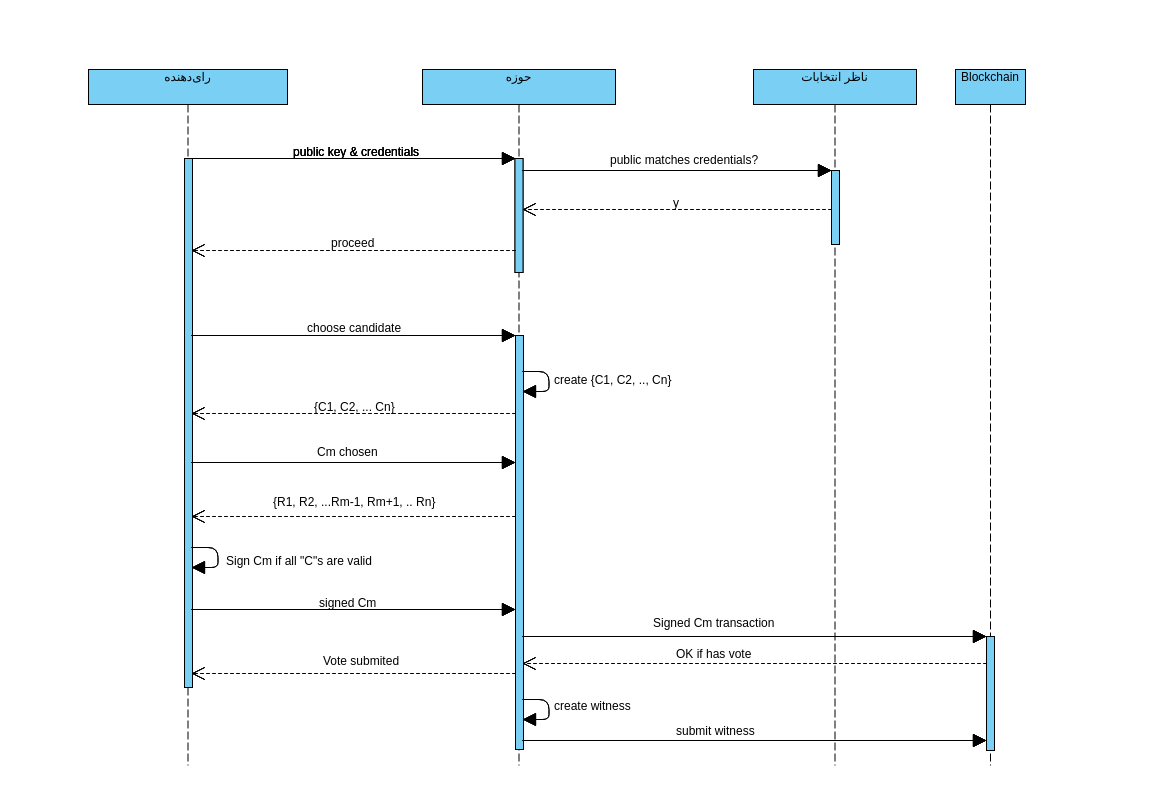
\includegraphics[width=1\linewidth]{seqdiag.png}
	\caption {فرایند ثبت رای در حوزه}
	\label{fig:seqdiag.png}
\end{figure}

\section{شمای کلی}
به طور کلی سیستم از تعدادی حوزه‌ تشکیل می‌شود که روی یک زنجیره‌ی قالبی توافق می‌کنند. همچین هر حوزه ممکن است بلوک‌ آماده شده و منتظر گرفتن تایید از بقیه‌ی حوزه‌ها داشته باشد، یا این که بلوکی از حوزه‌ی دیگری گرفته باشد که باید بررسی و امضا کند، شکل \ref{fig:bigpic} شمای کلی درشت‌دانه‌ی سیستم را نشان می‌دهد.
\\
بلوک ابتدایی این زنجیره‌ی قالبی به ازای هر فرد واجد شرایط یک کلید عمومی و یک رای‌دارد. همچنین یک آدرس خروجی به ازای هر کاندیدا وجود دارد که تعداد رای‌هایی که به آن آدرس فرستاده شده باشند رای‌های آن‌ کاندیداست. 
 
\begin{figure}[th]
	\centering
	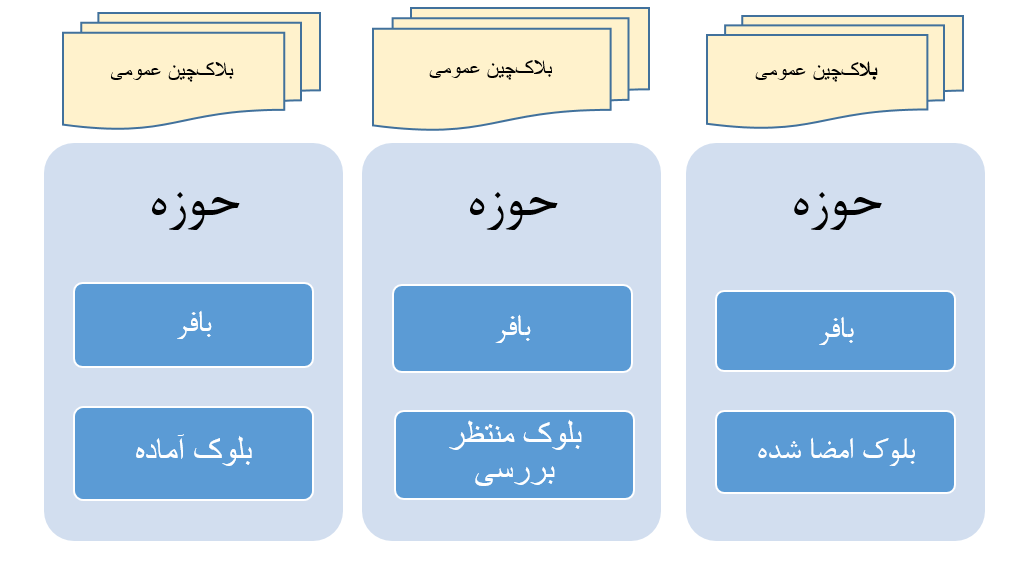
\includegraphics[width=1\linewidth]{blockchain.PNG}
	\caption {شمای منطقی سیستم}
	\label{fig:bigpic}
\end{figure}

\subsection{اضافه شدن بلوک}
می‌دانیم که در هر بلوک ثبت‌شده در زنجیره‌ی قالبی تعدادی از دو مدل تراکنش‌های ثبت و شمارش داریم، همچنین هش بلوک قبلی را نیز برای اطمینان از تغییر نکردن بلوک‌های قبلی نگه‌می‌داریم. مسئله‌ای که در اینجا باقی می‌ماند نحوه‌ی توافق روی یک زنجیره‌ی قالبی است. در این تحقیق از یک زنجیره‌ی قالبی عمومی و بسته استفاده می‌کنیم.
\\
هر حوزه یک بافر برای نگه‌داری تراکنش‌های مربوط به آرا دارد که قبل از ثبت در زنجیره‌ی قالبی که آن را تبدیل به یک بلوک می‌کند. برای اضافه شدن هر تراکنش روی زنجیره‌ی قالبی باید حداقل نصف به علاوه‌ی یکی از حوزه‌ها روی آن توافق کنند. هر حوزه برای توافق بررسی می‌کند که که تراکش‌های مربوط به رای دادن و شاهد‌های ثبت شده در بلوک جدید درست باشند و هش بلوک قبلی نیز در بلوک صحیح باشد. هر حوزه‌ی زنجیره‌ی قالبی را با امضای دیجیتال خود تایید می‌کند. 

\subsection{مقادیر اولیه  برای \lr{ZK-SNARK}}
همانطور که قبلا اشاره کردیم برای استفاده از روش \lr{ZK-SNARK} برای ایجاد‌ شاهد‌های بی‌دانش احتیاج به توافق روی نقاط اولیه‌ای روی یک \lr{elliptic curve} داریم. برای انجام این کار از روش ارائه شده در تحقیق 
\cite{multipartyparams}
استفاده می‌کنیم. در این روش برای ایجاد نقاط اولیه از تقسیم مسئله‌ بین افراد توافق‌کننده استفاده می‌شود، به صورتی که حاصل ضرب اطلاعات همه‌ی افراد نقاط اولیه را تشکیل می‌دهند و برای لو رفتن آن باید تمامی حوزه‌ها تبانی کنند. در این روش خود برای ایجاد پارامترها از یک حالت خاص اثبات‌های بی‌دانش استفاده می‌شود. 
\subsection{توافق}
 در زنجیره‌ی قالبی‌های عمومی معمولا یک مسئله‌ در توافق حالت‌هاییست که زنجیره‌ی قالبی دو شاخه می‌شود، یعنی دو مدل از زنجیره‌ی قالبی وجود داشته باشد که هر کدام را قسمتی از شبکه به عنوان زنجیره‌ی قالبی درست بشناسند. در بسیاری از ارزهای دیجیتال طولانی‌ترین زنجیره‌ی قالبی از نظر تعداد بلوک‌ها همواره به عنوان نسخه‌ی درست شناخته می‌شود اما در یک سیستم رای‌گیری این کار باعث کم شدن رای‌‌ می‌شود و این ریسک قابل قبولی نیست. 
 
\subsubsection{قضیه‌ی \lr{CAP}}
این قضیه‌ی معروف 
\cite{CAP}
اثبات می‌کند که در یک دیتابیس توزیع‌شده - مانند یک زنجیره‌ی قالبی - در هر بازه‌ای حداکثر می‌توان دو شرط از سه شرط همخوانی 
\LTRfootnote{Consistency}
، دردسترس بودن 
\LTRfootnote{Availability}
و تحمل قسمت‌شدن
\LTRfootnote{Partition tolerance}
را می‌توانند داشته باشند.با توجه به این که هیچ زمانی نمی‌توانیم روی درستی شبکه حساب کنیم سیستم‌ ما در حال \lr{CP} عمل می‌کند. معمولا در سیستم‌ها مبتنی بر زنجیره‌ی قالبی از روش‌های  که گارانتی می‌کنند که همه‌ی نودها در نهایت به همخوانی می‌رسند
\LTRfootnote{Eventual consistency}.
اما در یک سیستمی که برای رای‌گیری استفاده می‌شود این مسئله می‌تواند خطر گم شدن تعدادی از آرا ایجاد کند و این خطر معقولی برای یک‌ سیستم‌ رای‌گیری الکترونیکی نیست.
\par
در زنجیره‌ی قالبی‌های عمومی معمولا از روش‌های اثبات کار و اثبات‌ سهم استفاده می‌شود که دسترس پذیری و تحمل قسمت‌شدن را به خوبی ارائه می‌کنند اما ممکن است شاخه‌های
\LTRfootnote{fork}
لحظه‌ای پیش بیاید و چند نسخه از زنجیره‌ی قالبی درست وجود داشته باشد، معمولا در این روش‌ها طولانی‌ترین زنجیره‌ی قالبی نسخه‌ی درست در نظر گرفته می‌شود و زنجیره‌ی قالبی‌های کوتاه‌تر حذف می‌شوند. از آن‌جایی که این کار در سیستم ما باعث از بین رفتن رای‌ می‌شود باید در روش دیگری استفاده کنیم.
\par
در این تحقیق سه روش برای تفاوق را بررسی می‌کنیم. روش اول \lr{Aura}
\cite{Aura}
 نام دارد. در این روش نود یک نود رهبر بلوک‌های جدید ارائه می‌کند و در طور زمان در دوره‌های مشخصی رهبر تغییر می‌کند. برای انتخاب زمان تغییر از ساعت \lr{unix} استفاده می‌شود که می‌تواند در اثر همگام
\lr{sync}
 نبودن ساعت نود‌های حاضر در شبکه در یک لحظه دو رهبر وجود داشته باشد. این باعث از بین رفتن همخوانی در سیستم می‌شود ولی سیستم همواره در دسترس خواهد بود. 
\par
روش دیگر \lr{Clique} 
\cite{Clique}
نام دارد. این روش شبیه \lr{Aura} عمل می‌کند با این تفاوت که برای همگامی نودها به جای استفاده از ساعت، از تعداد بلوک ثبت شده در زنجیره‌ی قالبی استفاده می‌شود، همچنین در این روش، نود‌هایی غیر از نود رهبر نیز می‌توانند بلوک جدید پیشنهاد کنند. این کار می‌تواند باعث ایجاد شاخه‌ در زنجیره‌ی قالبی شود اما در طول زمان با تغییر رهبر یکی از دو شاخه حذف خواهد شد. این روش نیز در نهایت به همخوانی می‌رسد اما ریسک حذف شدن رای را سیستم وارد می‌کند.
\par

راه‌حلی در در پروتکل ارائه شده در این تحقیق برای این موضوع استفاده کردیم
\lr{PBFT}
\LTRfootnote{Practical Byzantine fault tolerance}
\cite{PBFT}
نام دارد. این روش هزینه‌ی محاسباتی بسیار کمتری از روش‌های مبتنی بر اثبات کار دارد و از نظر مقیاس پذیری
\cite{PBFperf}
نیز بسیار بهتر عمل می‌کند.

\begin{table}[th!]
	\begin{center}
		%		\def\arraystretch{2}
		\caption{روش توافق}
		\begin{tabular}{|c|c|c|c|}
			\hline
			& هم‌خوانی & دردسترس بودن & تحمل تقسیم شدن \\
			\hline
		 اثبات کار & همخوانی‌ در نهایت & دارد(اما ممکن است بلوک حذف شود) & دارد \\
			\hline
		 اثبات سهم & همخوانی‌ در نهایت & دارد(اما ممکن است بلوک حذف شود) & دارد \\
\hline
		 Aura & گارانتی نمی‌کند & دارد & دارد \\
\hline
		 Clique & همخوانی‌ در نهایت & دارد(اما ممکن است بلوک حذف شود) & دارد \\
\hline
PBFT & دارد & در صورت تقسیم شدن ندارد & دارد \\
\hline
		\end{tabular}
		\label{tab:cons}
	\end{center}
\end{table}


\subsubsection{\lr{Practical Byzantine Faul Tolerance}}

 در این روش در ابتدای رای‌گیری حوزه‌ها در یک زنجیره‌ی اولویت چیده می‌شوند و برای ثبت هر بلوک جدید، بلوک آماده‌شده را به رهبر (حوزه‌ای با بیشترین اولیت) داده می‌شود و حوزه آن‌ را به تمامی حوزه‌های دیگر ارسال می‌کند. سپس تمامی حوزه‌های دیگر بعد از تایید نتیجه را برای هم ارسال می‌کنند و در صورت موفقت آن را ثبت می‌کنند، بعد از تایید نتایج برای حوزه‌ی ابتدایی ارسال شده و ثبت نهایی می‌شود.
 \par
 همچنین بعد از اضافه شدن هر بلوک حوزه‌ی رهبر تغییر می‌کند و به نفر بعدی در زنجیره‌ی اولیت می‌رسد. همچنین در صورت جواب ندادن حوزه‌ی رهبر در مدت زمان مشخص یا جواب‌های غلط دادن مسئولیت به نفر بعدی منتقل می‌شود. 
 
 \begin{figure}[h!]
 	\centering
 	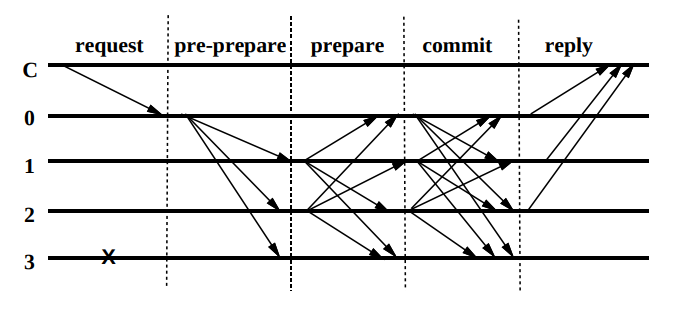
\includegraphics[width=1\linewidth]{PBFT.png}
 	\caption {روش \lr{PBFT}}
 	\label{fig:PBFT}
 \end{figure}
 
 \par
  در این روش حداکثر تعداد تعداد حوزه‌ای که باید خطاکار باشند تا بلوک اشتباهی در زنجیره‌ی قالبی ثبت شود برای 
$3f + 1$
حوزه $f$ حوزه‌است.
 این تعداد حوزه‌ی خراب‌کار می‌توانند بلوک‌های اشتباهی ثبت کنند اما به دلیل استفاده از امضای دیجیتال بعد از اتمام رای‌گیری با بررسی درستی بلوک‌های ثبت شده در زنجیره‌ی قالبی بلوک‌های خطا به سادگی قابل شناسیایی هستند. در همچین شرایطی چون نمی‌توان از تعداد رای‌دهندگانی که رای‌ آن‌ها ثبت نشده اطمینان پیدا کرد نتایج رای‌گیری باید مردود محسوب شود. 
 \par
 در روش \lr{PBFT} اثبات می‌شود 
 \cite{bftcap}
 تا زمانی که کمتر از یک سوم حوزه‌ها خطاکار باشند هیچ زمانی دو نسخه‌ی مستقل از زنجیره‌ی قالبی توسط حوزه‌ها تایید نمی‌شود. به عبارت دیگر این روش به طور کامل هم‌خوانی و توانایی قسمت‌شدن را دارد.
 \par
 لازم به ذکر است که در این حالت سیستم همواره دردسترس نیست. به این معنی که ممکن است موقعیتی پیش بیاید که یک حوزه به دلیل قطع شدن شبکه از بقیه‌ی حوزه‌ها نتواند بلوک جدید ثبت کند، اما می‌تواند در بافر خود اطلاعات آرا را نگه دارد و زمان اتصال به شبکه بلوک جدید را بسازد و ثبت کند.
\cchapter{تحلیل و ارزیابی}
در این فصل به تحلیل و بررسی روش ارائه شده و مقایسه‌ی این روش با روش‌های دیگر رای‌گیری می‌پردازیم. در ابتدا با بررسی جزییات پیاده‌سازی تست شده در روش می‌پردازیم و بعد از بررسی نحوه‌ی ارضای شرایط رای‌گیری ایده‌آل، این روش را در قیاس با روش‌های دیگر از نظر هزینه و میزان اعتماد مورد نیاز بررسی می‌کنیم. 
\par

\section{پیاده سازی}

در پیاده‌سازی این کار نیازمندی ابزاری برای ایجاد یک زنجیره‌ی قالبی خصوصی با روش تفاوق \lr{PBFT} هستیم. برای این کار از 
\lr{hyperledger fabric} \LTRfootnote{https://www.hyperledger.org/projects/fabric}
که یک بستر قراردادهای هوشمند است استفاده شده است. 
\lr{hyperledger fabric}
توسط شرکت \lr{IBM} طراحی شده و توسط \lr{Linux Foundation} نگهداری می‌شود. این پروژه یک زنجیره‌ی قالبی خصوصی ارائه می‌کند که قسمت‌های مختلف آن مانند روش توافق به سادگی قابل تغییرند. این ابزار به کمک \lr{NodeJS} نوشته شده است و به کمک داکر 
\LTRfootnote{Docker}
به سادگی تعدادی نود با یک بلاک‌چین خصوصی ارائه می‌کند. همچنین به کمک نوشتن قرارداد‌های هوشمند بر روی این بستر می‌توانیم حوزه‌های مورد نیاز را ایجاد کنیم. 
\par 
مسئله‌ی بعدی روش ایجاد اثبات‌های بی‌دانش است. برای ایجاد تراکنش‌های شمارش نیاز به اثبات‌های بی‌دانش داریم. برای برای ساخت اثبات‌های بی‌دانش از کتاب‌خانه‌ی 
\lr{libsnark}\LTRfootnote{https://github.com/scipr-lab/libsnark}
استفاده شده است. این کتاب‌خانه از الگوریتم پینوکیو را با زبان \lr{C++} پیاده کرده است و توسط \lr{Zcash} - یکی از بزرگ‌ترین ارز‌های دیجیتال با توانایی تراکنش ناشناس - نیز برای ساخت اثبات استفاده شده است.
\par
در فرایند کامپایل این کتاب‌خانه از تنظیمات موجود در جدول \ref{tab:libsnark} استفاده شده است. 
\begin{table}[h!]
	\begin{center}
		%		\def\arraystretch{2}
		\caption{تنظیمات \lr{libsnark}}
		\begin{tabular}{|c|c|c|}
			\hline
			نام متغیر& مقدار & توضیحات \\
			\hline
			CURVE & \lr{ALT\_BN128} & مدل خم مورد استفاده با ۱۲۸ بیت امنیت \\
			\hline
			MULTICORE & ON & استفاده از چند هسته برای موازی سازی \\
			\hline
			USE\_PT\_COMPRESSION & OFF & سرعت بالاتر در ازای حجم شاهدهای بزرگتر \\
			\hline
			PROFILE\_OP\_COUNTS & OFF & شمارش تعداد فعالیت روی خم 
			 \\
			 \hline
		\end{tabular}
		\label{tab:libsnark}
	\end{center}
\end{table}
\\
بقیه‌ی تنظیمات کتاب‌خانه در حالت پیش‌فرض استفاده شده است.

\section{نزدیکی به رای‌گیری ایده‌آل}
در این بخش نیازمندی‌های رای‌گیری ایده‌آل را دوره می‌کنیم و می‌بینیم که سیستم ارائه شده چگونه هر کدام از نیاز‌مندی‌ها را رفع می‌کند.

\begin{itemize}
	\item 
	می‌دانیم که هر شخصی حداکثر یک رای‌ می‌تواند بدهد چون که در حساب کلید عمومی آن فرد دقیقا یک رای در ابتدای رای‌گیری وجود دارد. از طرفی می‌دانیم که سیستم مانع رای دادن فردی نمی‌شود چرا که رای‌دهنده می‌تواند بررسی کند که رای‌ او در زنجیره‌ی قالبی مصرف شده باشد.
	\item 
	می‌دانیم کسی نمی‌تواند به جای دیگری رای دهد، چرا که برای رای دادن هم نیاز به دسترسی به کلیدخصوصی دارد و هم کلید عمومی فرد با اطلاعات شناسایی او در حوزه مقایسه می‌شود.
	\item 
	با اضافه شدن گزینه‌ی ممتنع و حفظ امنیت فیزیکی حوزه‌ی رای‌گیری می‌توانیم اطمینان حاصل کنیم که کسی مجبور به رای‌ دادن نمی‌شود.
	\item 
 هیچ کسی مجبور به رای‌دادن به شخص خاصی نمی‌شود چرا که راهی برای چک کردن رای‌ فرد بعد از فرایند رای‌گیری وجود ندارد، در نتیجه به دلیل امن بودن حوزه‌ی رای‌گیری، رای‌دهنده همواره می‌تواند به کاندیدای دلخواه خود رای‌ دهد ولی این عمل را انکار کند.
	\item 
	در انتهای انتخابات می‌توانیم به سادگی با بررسی تعداد تراکنش‌های ثبت و شمارش از درستی شمارش آرا اطمینان حاصل کنیم. هر شخصی نیز با بررسی این که عمل ثبتی برای او در زنجیره‌ی قالبی وجود دارد می‌تواند از شمارده شدن رای خود اطمینان حاصل کند.
	\item 
	نتیجه‌ی آرا ناشناس  باقی می‌ماند چرا که تراکنش‌های ثبت کورکورانه امضا می‌شوند حتی خود رای‌دهنده با وجود از اطمینان از نتیجه‌ی رای راهی برای چک کردن نتیجه‌ی برگه‌ی رایش بعد از انتخابات ندارد.
	\item 
	در هر زمانی که یک بلوک جدید در زنجیره‌ی قالبی ثبت شود می‌توان با با استناد به حساب‌های کاندیداها از نتیجه‌ی آن لحظه‌ی انتخابات مطلع شد. در صورتی هم که مجری انتخابات نخواهد که نتایج لحظه‌ای را منتشر کند می‌تواند زنجیره‌ی قالبی را تا پایان انتخابات بسته نگه دارد. 
\end{itemize}




\section{مقایسه با کارهای مشابه}
در این بخش به مقایسه‌‌ی روش رای‌گیری ارائه شده با تحقیقات دیگر در این زمینه می‌پردازیم . این مقایسه را از چند جنبه‌ی نحوه‌ی اطمینان از ثبت رای، ناشناسی آرا،  سطح اعتماد مورد نیاز و  هزینه‌ی انتخابات بررسی می‌کنیم. 
\subsection{روش‌های رای‌گیری دیگر}
برای مقایسه سیستم‌های رای‌گیری زیر را بررسی می‌کنیم:
\begin{itemize}
	\item 
	\textbf{رای‌گیری سنتی}:
	این روش به عنوان خط مبنای تحقیق بررسی می‌شود، در این روش از سیستم‌های الکترونیکی برای رای‌گیری استفاده نمی‌شود. این روش در بخش ۱.۲ توصیف شده است. 
	\item \textbf{رای‌‌گیری الکترونیک بدون زنجیره‌ی قالبی}:
	در این روش، رای‌گیری الکترونیک متمرکز را بررسی می‌کنیم، چرا که سیستم‌های رای‌گیری توزیع‌شده‌ی بدون زنجیره‌ی قالبی به به کاربرد عمومی نرسیدند. در این سیستم‌ها اطلاعات رای‌دهندگان و نتیجه‌ی رای آن‌ها به دلیل نیاز به روش ردگیری به طور کامل ثبت می‌شود اما در فرایند ثبت رای تفاوت چندانی با سیستم‌های سنتی ندارند.
 	\item \textbf{\lr{VoteBook}}
 	این سیستم را به عنوان مصداقی از سیستم‌های رای‌گیری با زنجیره‌ی قالبی خصوصی بررسی می‌کنیم. 
 	در این سیستم از یک‌ زنجیره‌ی قالبی که می‌توان در حالت خصوصی یا عمومی از استفاده کرد برای ثبت آرا استفاده می‌شود. 
\end{itemize}
\par
 	 سیستم‌ معروف \lr{VoteWatcher} نیز فعالیت‌های بسیاری در این زمینه داشته اما به دلیل عمومی نبودن اطلاعات پیاده‌سازی این سیستم‌، از مقایسه‌ی آن خود‌داری می‌کنیم. 
 	 \\
 	 همچنین از آن‌جایی که روش‌های رای‌گیری به کمک یک زنجیره‌ی قالبی عمومی و یا روش‌های توزیع‌شده بدون زنجیره‌ی قالبی به دلیل مشکلات مقیاس‌پذیری توانایی استفاده شدن در انتخابات‌های بزرگ(بیش از چند هزار نفر) را ندارند از بررسی این نوع سیستم‌ها صرف نظر می‌کنیم.
 	 \\
 	 همچنین روش مورد استفاده در \lr{Follow my Vote} از لحاظ روش پیاده‌سازی شباهت زیادی به \lr{VoteBook} دارد ولی به جای حوزه‌ی رای‌گیری از یک برنامه در کامپیتور شخصی یا تلفن هوشمند استفاده می‌کند. این تصمیم باعث سادگی فرایند رای‌گیری برای بعضی از رای‌دهندگان می‌شود اما دو مشکل بزرگ ایجاد می‌کند که باعث شده از مقایسه‌ی آن خودداری کنیم. اولین مشکل کاهش دسترسی‌پذیری این سیستم برای افرادی که دسترسی به اینترنت ندارند است و دومین مشکل این است که بدون وجود یک حوزه‌ی امن، راهی وجود ندارد تا اطمینان حاصل کنیم که رای‌دهنده مجبور به رای‌دادن به کاندیدای خاصی نشده است.
\subsection{اطمینان از شمارش درست}
شاید مهمترین شرط برگزاری یک انتخابات میزان اطمینان از شمارش درست آرا در آن‌ باشد. در این بخش به بررسی نجوه‌ی شمارش آرا در روش‌های مختلف می‌پردازیم. 
\par
در روش سنتی برای شمارش آرا بعد از اتمام انتخابات برگه‌های رای‌ موجود در صندوق‌ها به مکانی منتقل می‌شوند و در آن‌ جا یا به روش انسانی و یا با استفاده از دستگاه‌های الکترونیکی شمارش می‌شوند. طبیعتا این مدل شمارش به دلیل دخالت انسانی احتمال خطای نسبتا بالایی دارد. همچنین برای اطمینان درستی شمارش یک حوزه، تنها روش شمارش کامل برگه‌های رای‌ آن حوزه است که هزینه‌ی آن معادل هزینه شمارش اولیه می‌باشد. 
\par 
در روش‌های رای‌گیری بدون زنجیره‌ی قالبی برای ثبت رای، اطلاعات کاربر به طور رمزشده به همراه نتیجه‌ی رای‌ او ثبت می‌شود. دلیل نگه‌داشتن اطلاعات رای‌دهنده توانایی رد‌گیری و بررسی درستی شمارش آرا است. در این سیستم‌ها شمارش رای‌گیری به صورت آنلاین اتفاق می‌افتد و هزینه‌ی چندانی ندارد، همچنین بررسی ناظر انتخابات هزینه‌ ناچیزی خواهد داشت. 
\par 
در سیستم \lr{VoteBook} و سیستم پیشنهادی این تحقیق نیز روال شمارش آرا تفاوت چندانی ندارد و هزینه‌ی اضافه‌ای برای شمارش آرا اضافه نمی‌کنند. اما در این دو روش با عمومی شدن زنجیره‌ی قالبی قبل یا در حین رای‌گیری رای‌دهندگان نیز می‌توانند از درستی شمارش آرا و شمرده شدن رای خود اطمینان حاصل کنند. 
\subsection{حریم خصوصی}
در روش سنتی برگزاری انتخابات با توجه به ناشناس بودن برگه‌های رای در صندوق رای‌گیری راهی برای فهمیدن نتیجه‌ی رای‌ یک فرد خاص نیست. البته با توجه به این که حوزه‌ی رای‌گیری برگه‌های رای را از قبل از انتخابات در دسترس دارد، این گزاره در صورتی صحیح است که حوزه یا شماره یا علامتی ناشناسی برگه‌های رای را از بین نبرده باشد.
\par 
در روش‌های رای‌گیری الکترونیک بدون زنجیره‌ی قالبی، با توجه به عمومی نشدن اطلاعات رای‌گیری اطلاعات محفوظ می‌مانند. در این روش نیز حوزه‌ی انتخابات که مسئولیت رمزکردن اطلاعات شخصی کاربر را دارد می‌تواند به حریم خصوصی آسیب بزند. همچینین برای جلوگیری از دو بار رای دادن یک کاربر باید مرکز مستقلی که اطلاعات رای‌گیری را ذخیره می‌کند نیز توانایی بازگشایی اطلاعات کاربر را داشته باشد در نتیجه این مرکز و تمامی افرادی که به اطلاعات آن دسترسی دارند نیز می‌توانند حریم خصوصی را نقض کنند. 
\par
در روش \lr{VoteBook} هر رای‌دهنده یک «شماره‌ی رای‌دهنده» دارد و بعد از رای دادن نیز یک «شماره‌ی رای» دریافت می‌کند. در ادامه هش شماره‌ی رای و شماره‌ی راه‌دهنده در زنجیره‌ی قالبی به عنوان رای‌دهنده ثبت می‌شود. در این روش علاوه بر حوزه، هر کسی که شماره‌ی رای و شماره‌ی رای‌دهنده را داشته باشد می‌تواند از نتیجه‌ی رای آن فرد آگاه شود. شماره‌های رای‌دهندگان در یک زنجیره‌ی قالبی خصوصی مستقل نگهداری می‌شود و هیچ وقت عمومی نمی‌شوند در نتیجه جدا از حوزه‌ی رای‌گیری فقط خود فرد (یا کسی که اطلاعات خصوصی او را از خودش دریافت کند) می‌تواند نتیجه‌ی رای فرد را بررسی کند. 
\par 
در روش پیشنهادی ما برای از بین بردن ریسک لو رفتن اطلاعات درست ثبت شدن رای در خود حوزه به کاربر اثبات می‌شود و چون خود کاربر تراکنش ثبت را کورکورانه امضا می‌کند بعد از فرایند ثبت رای راهی برای پیدا کردن نتیجه‌ی رای فرد وجود ندارد. در این روش نیز مانند همه‌ی روش‌های ممکن در رای‌گیری حوزه‌ی خطاکار می‌تواند در حین دریافت رای نتیجه‌ی آن را جداگانه ثبت کند و از این روش به حریم خصوصی آسیب بزند اما با توجه به این که تمامی بلوک‌ها توسط حوزه‌ها امضا شده‌اند در صورت نقض حریم خصوصی به سادگی حوزه‌ی خطاکار مشخص می‌شود.

\subsection{هزینه برگزاری}
در این بخش هزینه‌ی برگزاری انتخابات با هر کدام از روش‌ها را از دید کاربر و از دید مجری انتخابات بررسی می‌کنیم.
\subsubsection{هزینه برای کاربر}
فرایند رای‌دادن کاربر در روش‌هایی که بررسی می‌کنیم به سه حالت خواهد بود:
\begin{itemize}
 \item 
 در روش‌ سنتی و رای‌گیری بدون زنجیره‌ی قالبی کاربر برای رای‌دادن صرفا نیاز کارت شناسایی دارد. کاربر با ارائه‌ی کارت شناسایی و بعد از بررسی شدن این که کاربر دو بار رای نداده رای خود را ثبت می‌کند. 
 \item 
 در رای‌گیری با زنجیره‌ی قالبی با هدف افزایش شفافیت و ایجاد اطمینان از شمارش درست آرا برای کاربر، هر کاربری نیاز به ثبت یک «هویت یکتا» در سامانه‌ی مربوط به انتخابات دارد. در \lr{VoteBook} این کار با شماره‌ی رای‌‌دهنده اتفاق می‌افتد و همچنین کاربر باید قبل از رای‌ دادن حوزه‌ی مد نظر خود را برای رای‌دادن مشخص کند. دلیل مشخص کردن حوزه این است که شماره‌ی رای‌دهندگان ممکن از قبل در حوزه ذخیره شده باشند.
 
 \item
 در سیستم ما نیز کاربر باید قبل از رای‌گیری یک کلید عمومی ثبت کند که برای فرایند رای‌گیری استفاده می‌شود. همچنین کاربر برای اطمینان از درست شمرده شدن رای خود می‌تواند از یک دستگاه هوشمند برای عمل امضای کورکورانه استفاده کند. کاربر می‌تواند از دستگاه‌های درون حوزه استفاده کند ولی با این کار باید اعتماد کند که حوزه رایش را به درستی ثبت کرده چرا که راهی برای اثبات درستی برنامه‌ی موجود در حوزه وجود ندارد.
 در ادامه فرایند مانند روش‌های 
\end{itemize}
\subsubsection{هزینه انتخابات برای مجری}
در روش سنتی انتخابات هزینه‌ی اولیه‌ای برای مجری ایجاد نمی‌شود اما در هر انتخابات جدا از هزینه‌ی ایجاد حوزه، هزینه‌ی تولید برگه‌ی رای فیزیکی و شمارش را باید تحمل کند. 
\\
در روش‌های رای‌گیری الکترونیک متمرکز جدا از حوزه هزینه‌ی اضافی معنی‌داری به مجری تحمیل نمی‌شود، اما دستگا‌ه‌های الکترونیکی نیازمند بررسی و ارتقا در طول زمان هستند.
\\
در \lr{VoteBook} یک سامانه‌ای برای ثبت و نگهداری اطلاعات محل رای‌گیری و شماره رای‌دهنده برای هر کاربر وجود دارد که خود این مسئله نیز نیازمند بررسی امنتی مداوم و ارتقا است. 
\\
در سیستم پیشنهادی ما نیز در هر انتخابات، مجری انتخابات باید توانایی عوض کردن یا ثبت کلید عمومی جدید را به رای‌دهندگان بدهد که خود این مسئله یک هزینه‌ی نگهداری به مجری اضافه می‌کند. 
\subsection{توانایی ردگیری خطا}
برای درستی انتخابات نیاز است که برای ناظر انتخابات راهی وجود داشته باشد تا از درستی برگزاری انتخابات اطمینان حاصل کند. با توجه به این که یک حوزه‌ی انتخابات خطاکار همواره می‌تواند بعضی رای‌ها را شمارش نکند و یا تلاش کند که رای جعلی تولید کند، در این بخض توانایی ردگیری همچین حملاتی را بررسی می‌کنیم.
در روال سنتی رای‌گیری با توجه به کاغذی بودن آرا و وصل نبودن برگه‌ی رای به کاربر، فراتر از بررسی تعداد آرا و مقایسه‌ی آن‌ها با تعداد برگه‌ی ثبت رای راهی برای بررسی درستی نتایج حوزه وجود ندارد. ایجاد برگه‌ رای‌های غلط هزینه‌ی اندکی ندارد ولی در انتخابات‌های حساس ممکن است به صرفه باشد و در صورت اتفاق افتادن همچین مسئله‌ای، راه‌حل سیستمی برای پیدا کردن مشکل وجود ندارد. همچینین در صورتی که بخشی از آرا توسط حوزه دور ریخته شود، ناظر انتخابات هیچ راهی برای فهمیدن این عمل ندارد و رای‌دهندگان عادی نیز روش برای فهمیدن این موضوع که رای آن‌ها شمرده نشده ندارند.
\par 
در سیستم‌های رای‌گیری الکترونیک بدون زنجیره‌ی قالبی نیز رای‌دهنده راهی برای اطمینان حاصل کردن رای‌‌دهنده از شمارش رایش وجود ندارد. همچنین راهی برای ناظر انتخابات برای تشخیص دادن رای‌هایی که فرستاده نشده‌اند وجود ندارد. با توجه به این که کاربر برای ارسال رای هیچ راه شناسایی مستقل از حوزه‌ای هم ندارد، ایجاد رای دروغین توسط حوزه هم ممکن است. 
\par 
در سیستم‌ \lr{VoteBook} برای ایجاد اطمینان از شمارش آرا تمامی رای‌ها شفاف ذخیره می‌شوند و هر کسی که با اطلاعات خصوصی خود می‌تواند بررسی کند که رای او به درستی ثبت شده است. ناظر انتخابات نیز می‌تواند رای‌های ثبت شده را با اطلاعات کاربرانی که باید در آن حوزه رای می‌دادند بررسی کند و به این صورت هیچ رای اشتباهی نمی‌تواند ثبت شود. اما یک حمله‌ای که حوزه‌ی خراب‌کار می‌تواند انجام دهد این است که رای کاربر را به عنوان رای ممتنع ثبت کند. در فرایند رای‌گیری با \lr{VoteBook} از کاربر پرسیده می‌شود که تحت فشار مجبور به رای دادن شده یا خبر، در صورت پاسخ بله کاربر شماره‌ی رای کاربر به عنوان رای ممتنع ثبت می‌شود و اطلاعات آرا ممتنع هیچ‌وقت به صورت عمومی منتشر نمی‌شوند اما با توجه به این که این اطلاعات در اختیار ناظر انتخابات خواهد بود حمله‌‌ی بزرگ به این روش به سادگی قابل تشخیص خواهد بود. 
\par 
در سیستم رای‌گیری ما نیز کاربر از درستی شمارش رای‌ ثبت‌شده‌ی خود در فرایند امضای کورکورانه آگاه می‌شود همچنین بعد از فرایند رای‌گیری نیز می‌تواند با بررسی زنجیره‌ی قالبی از ثبت رای‌ خود (ولی نه نتیجه‌ی آن) مطمئن شود. از آن‌جایی که تمامی رای‌ها نیازمند امضای دیجیتال رای‌دهندگان هستند راهی برای ایجاد رای‌های دروغین توسط یک حوزه نیز وجود ندارد. از طرفی ناظر انتخابات می‌تواند با بررسی تساوی تعداد تراکنش‌ها ثبت و شمارش ثبت شده در زنجیره‌ی قالبی رفتار حوزه را تحلیل کند. در صورت پیدا کردن خطا از یک حوزه راهی برای پیدا کردن کاربری که رای او شمرده نشده و نتیجه‌ی رای او نخواهد بود.



\begin{table}[h]
	\begin{center}
				\def\arraystretch{2}
		\caption{مقایسه‌ی روش‌های رای‌گیری}
		\begin{tabular}{|c|c|c|c|c|}
			\hline
			معیار & روش سنتی & بدون زنجیره‌ی قالبی & \lr{VoteBook} & روش پیشنهادی\\
			\hline
شمارش درست & \vtop{\hbox{\strut احتمال خطای انسانی و }\hbox{\strut هزینه‌ی زیاد}} & کم هزینه & کم هزینه & کم هزینه \\ 
			\hline
خطر نقض حریم خصوصی &  حوزه &  حوزه‌ و مرکز & حوزه و رسید رای &  حوزه \\
			\hline
			هزینه‌ی برگزاری & زیاد & کم & متوسط & متوسط \\
			\hline
			هزینه‌ی کاربر & کم & کم & متوسط & متوسط \\
			\hline
			ردگیری خطای حوزه & ناممکن & ناممکن & ممکن & ممکن \\
			\hline
		\end{tabular}
		\label{tab:compare}
	\end{center}
\end{table}


\cchapter{نتیجه‌گیری و کارهای آتی}
\section{نتیجه‌گیری}
تحقیقات در راستای ایحاد رای‌گیری امن قبل از فراگیری تکنولوژی زنجیره‌ی قالبی بسیار نادر بود اما با فراگیری این تکنولوژی و کاربرد‌های آن تحقیقات جدید و خلاقانه‌ای در این زمینه انجام شده است. در این تحقیق روش‌های استفاده شده در رای‌گیری‌های الکترونیکی را بررسی کردیم. سپس زنجیره‌ی قالبی را به عنوان یک ابزار برای کاهش نیاز به شخص مورد اعتماد در رای‌گیری استفاده کردیم تا یک رای‌گیری با توانایی ردگیری خطا از مجری انتخابات و حوزه‌ها بسازیم. همینطور نشان دادیم که کم کردن نیاز به اعتماد لزوما به معنی کاهش حریم خصوصی نیست و با استفاده از اثبات‌های بی‌دانش پروتکل‌ امنی برای شمارش رای بدون به خطر انداختن حریم خصوصی رای‌دهنده ارائه دادیم. 
\par 
با استفاده از این روش رای‌گیری می‌توان یک رای‌گیری الکترونیکی امن برگزار کرد که علاوه بر هزینه‌ی بسیار کمتر از روش‌های سنتی، باعث افزایش اطمینان رای‌دهندگان و ناظران انتخابات به درستی آن نیز می‌شود. 

\section{کار‌های آتی} 
روش توافق استفاده شده در این تحقیق به ما اطمینان می‌دهد که زنجیره‌ی قالبی موجود در حوزه‌ها همواره با هم همخوان می‌ماند. این ویژکی برای کاربرد ما بسیار مناسب است اما باعث می‌شود که در صورت خطاکار بودن بیش از یک سوم حوزه‌‌ها کل فرایند رای‌گیری - حتی برای حوزه‌های درست‌کار - متوقف شود. استفاده از روش‌هایی مانند \lr{Clique} که در نهایت همخوان می‌شوند یا تغییر در ساختار زنجیره‌ی قالبی مورد استفاده به گونه‌ای که بتواند چند زنیجره‌ی درست را با هم تبدیل به یک زنجیره کند باعث می‌شود حتی در صورتی که  حتی نیمی از حوزه‌ها خطاکار باشند رای‌گیری برای بقیه‌ی حوزه‌ها درست انجام شود. این تغییر می‌تواند به امنیت و مقیاس‌پذیری روش انتخابات کمک شایانی کند. 





